\documentclass[a4paper,12pt]{report}

% Pacotes (mantidos do template original do Insper, adequado para ABNT)
\usepackage[utf8]{inputenc}
\usepackage[T1]{fontenc}
\usepackage{graphicx}
\usepackage{amsmath}
\usepackage{amsfonts}
\usepackage{amssymb}
\usepackage{fancyhdr}
\usepackage{hyperref}
\usepackage{longtable}
\usepackage{tocbibind}
\usepackage{changepage}
\usepackage{geometry}
\usepackage{setspace}
\usepackage[portuguese]{babel}
\usepackage{caption}
\usepackage{ifthen}
\usepackage{times}
\usepackage[alf]{abntex2cite}
\usepackage[titles]{tocloft}
\usepackage{titlesec}
\usepackage{booktabs}

% Margens ABNT NBR 14724: superior 3cm, inferior 2cm, esquerda 3cm (encadernação), direita 2cm
\geometry{top=3cm, bottom=2cm, left=3cm, right=2cm}
\setlength{\parindent}{1.25cm}
\onehalfspacing

\renewenvironment{abstract}{
    \begin{center}
        \textbf{\abstractname}
    \end{center}
    \begin{quote}
}{\end{quote}}

\titleformat{\chapter}[hang]
  {\normalfont\huge\bfseries}{\thechapter}{0.25em}{}

\addto\captionsportuguese{\renewcommand{\contentsname}{Sumário}}
\addto\captionsportuguese{\renewcommand{\bibname}{Referências}}

\title{Alterações textuais nas notas explicativas de dívida e a incorporação de informações pelo mercado brasileiro: evidências das notas de empréstimos, financiamentos e debêntures}
\author{Jonathan Mark Miranda Buscariolli Majoni}
\date{\the\year}
\newcommand{\advisor}{Ruy Monteiro Ribeiro}
% \newcommand{\coadvisor}{}

\begin{document}
\selectlanguage{portuguese}

\makeatletter

\begin{titlepage}
    \begin{minipage}[t]{0.35\textwidth}
        \raggedright
        
\includegraphics[width=0.7\textwidth]{Logo_Insper.png}
    \end{minipage}

    \vspace*{1.5cm}
    \centering
    {\large INSPER, INSTITUTO DE ENSINO E PESQUISA}\\[3cm]

    {\large \@author}\\[3cm]

    {\Large \textbf{\@title}}

    \vfill
    {\large São Paulo}\\
    {\large \the\year}
\end{titlepage}
\newpage

\begin{titlepage}
    \centering
    {\large \@author}\\[3cm]
    {\Large \textbf{\@title}}\\[3cm]

    \begin{adjustwidth}{7cm}{0cm}
        Dissertação apresentada ao Programa de Mestrado Profissional em Economia do Insper Instituto de Ensino e Pesquisa, como requisito parcial para obtenção do título de Mestre.

        \vspace*{0.5cm}
        Orientador(a): \advisor
        \ifcsname coadvisor\endcsname
            \\[0.25cm] Coorientador: \coadvisor
        \fi
    \end{adjustwidth}

    \vfill
    {\large São Paulo}\\
    {\large \the\year}
\end{titlepage}
\newpage

% Na versão final: Ficha catalográfica (biblioteca) e Folha de aprovação (pós-defesa) entram aqui.
% Não incluídas nesta versão por dependerem de processos institucionais externos.

\thispagestyle{empty}
\newpage

\renewcommand{\abstractname}{Resumo}
\begin{abstract}
    Este estudo investiga se as alterações textuais ano a ano nas notas explicativas de empréstimos, financiamentos e debêntures das demonstrações financeiras anuais de empresas não financeiras listadas na B3 carregam conteúdo informacional incremental sobre o retorno anormal futuro das ações, mesmo após controlar pelas mudanças nos fundamentos econômico-financeiros da empresa. A amostra final compreende 111 empresas não financeiras listadas na B3 -- as 66 constituintes atuais do Ibovespa mais 45 empresas que integraram o índice em algum momento entre 2015 e 2024 mas não integram mais, incluídas para corrigir o viés de sobrevivência --, no período de 2015 a 2024. A mudança textual é medida por TF-IDF e similaridade de cosseno entre o texto da nota de um exercício e a do exercício anterior, seguindo a abordagem de \citeonline{cohen2020} e \citeonline{brown2011}. O retorno anormal é medido como o resíduo fora da amostra de um modelo de quatro fatores (mercado, tamanho, valor e momento) estimado por empresa, acumulado numa janela de doze meses e ajustado por winsorização; os controles seguem uma grade pré-especificada de blocos cumulativos (fundamentos de nível, mudanças contemporâneas nesses fundamentos, e determinantes de risco e retorno esperado), estimada em painel com efeitos fixos de empresa e ano e erros-padrão agrupados por empresa. [Completar com principais resultados quando disponíveis.]
\end{abstract}

\noindent
\textbf{Palavras-chave:} notas explicativas; análise textual; TF-IDF; retorno anormal; BHAR; modelo de quatro fatores; dados em painel; disclosure; consenso de estimativas.
\thispagestyle{empty}
\newpage

\renewcommand{\abstractname}{Abstract}
\begin{abstract}
    This study investigates whether year-over-year textual changes in the explanatory notes on loans, financing, and debentures in the annual financial statements of non-financial companies listed on B3 carry incremental informational content about firms' future abnormal stock returns, even after controlling for changes in the firm's economic and financial fundamentals. The final sample comprises 111 non-financial companies listed on B3 -- the 66 current constituents of the Ibovespa index plus 45 companies that were index constituents at some point between 2015 and 2024 but no longer are, included to correct for survivorship bias -- over the 2015--2024 period. Textual change is measured via TF-IDF and cosine similarity between the note's text in a given fiscal year and the previous year, following the approach of \citeonline{cohen2020} and \citeonline{brown2011}. Abnormal returns are measured as the out-of-sample residual from a firm-level four-factor model (market, size, value, and momentum), accumulated over a twelve-month window and adjusted via winsorization; controls follow a pre-specified grid of cumulative blocks (level fundamentals, contemporaneous changes in those fundamentals, and risk/expected-return determinants), estimated in a panel with company and year fixed effects and firm-clustered standard errors. [To be completed with the main results once available.]
\end{abstract}

\noindent
\textbf{Keywords:} explanatory notes; textual analysis; TF-IDF; abnormal returns; BHAR; four-factor model; panel data; disclosure; analyst consensus estimates.
\thispagestyle{empty}
\newpage

\tableofcontents
\thispagestyle{empty}
\newpage

\chapter{Introdução}

\section{Pergunta de pesquisa e objetivos}

A questão que este estudo busca responder é: as alterações textuais nas notas explicativas de dívida das empresas brasileiras carregam informação que são posteriormente incorporadas aos preços das ações pelo mercado?

Mais especificamente, em que medida as alterações textuais entre exercícios consecutivos, medidas por TF-IDF e similaridade de cosseno, nas notas de empréstimos, financiamentos e debêntures das demonstrações financeiras anuais de empresas não financeiras listadas na B3 estão associadas ao retorno anormal acumulado nos 12 meses seguintes à divulgação, depois de controlar pelas mudanças nos fundamentos econômico-financeiros da empresa? Como análise complementar, o estudo também verifica se essa mesma mudança textual se associa à revisão do consenso de previsões de lucro por ação (EPS) dos analistas depois da divulgação.

\textbf{Objetivo geral:} analisar se as alterações textuais entre exercícios consecutivos nas notas de empréstimos, financiamentos e debêntures carregam conteúdo informacional incremental para explicar os retornos anormais futuros de empresas não financeiras listadas na B3.

\textbf{Objetivos específicos:}
\begin{itemize}
    \item Extrair e organizar as notas de empréstimos, financiamentos e debêntures das DFPs anuais das empresas da amostra.
    \item Medir a similaridade textual entre a nota de cada exercício e a do exercício anterior, usando TF-IDF e cosseno.
    \item Testar se essa mudança textual se relaciona com o retorno anormal acumulado nos 12 meses seguintes à divulgação.
    \item Verificar se essa relação se mantém depois de controlar por alavancagem, rentabilidade, tamanho, retorno passado e outros fundamentos.
    \item Como análise complementar, testar se a mudança textual também se associa à revisão do consenso dos analistas depois da divulgação.
    \item Comparar o resultado obtido no recorte da nota de dívida com o resultado das mesmas hipóteses aplicadas a áreas de divulgação textual mais amplas e já mais exploradas na literatura internacional (conjunto completo de notas, Relatório da Administração, Fatores de Risco).
\end{itemize}

\section{Hipóteses}
\label{sec:hipoteses}

\textbf{H1}: as alterações textuais entre exercícios nas notas de empréstimos, financiamentos e debêntures estão associadas ao retorno anormal futuro das ações, mesmo depois de controlar pelas mudanças observáveis nos fundamentos da empresa.

Optou-se por manter essa hipótese sem direção definida de propósito. Uma mudança grande no texto pode originar de uma notícia ruim, como quebra de covenant ou dificuldade de refinanciamento, como também pode originar de uma notícia boa, como alongamento de prazo, redução de taxa ou quitação de dívida. Não se pode assumir de antemão que mudança sempre representa um impacto negativo. Essa leitura é consistente com \citeonline{brown2011}: a motivação central da medida de modificação textual dos autores não presume o sinal da mudança econômica subjacente. O argumento é que uma seção narrativa pouco modificada é pouco informativa após ``mudanças econômicas significativas'' na empresa, sem qualificar se essas mudanças são favoráveis ou desfavoráveis, e o teste principal do estudo usa a \emph{magnitude} da reação de preço ao texto modificado, não sua direção.

\textbf{H1a} (opcional, exploratória): empresas com maior mudança textual nas notas de dívida apresentam retorno anormal futuro menor, na linha do que ``Lazy Prices'' encontra para o mercado americano. Essa hipótese só se sustenta se a mudança estiver concentrada em notícia desfavorável, então é tratada como teste adicional, não como hipótese central da dissertação.

\textbf{H2} (complementar): as alterações textuais nas notas de dívida também se associam à revisão do consenso de EPS dos analistas depois da divulgação.

\section{Estrutura da dissertação}

[PLACEHOLDER - Escrever após terminar a dissertação]

\chapter{Referencial Teórico e Revisão de Literatura}

\section{Assimetria informacional e divulgação corporativa}

A base teórica mais geral é a existência de assimetria de informação entre os administradores, que acompanham de perto a operação da empresa, e os investidores de fora, que dependem do que é publicado. \citeonline{diamond1991} mostram que divulgação pública reduz a assimetria entre investidores informados e não informados, o que pode aumentar a liquidez e reduzir o custo de capital da empresa. \citeonline{healy2001}, numa revisão bem conhecida da literatura de disclosure, organizam as demonstrações financeiras, a auditoria, os intermediários de informação e as divulgações voluntárias como os mecanismos principais pelos quais o mercado tenta resolver esses problemas de informação e de agência.

Aplicando isso a esta pesquisa, não basta a empresa divulgar o saldo total da dívida. Informação sobre vencimento, taxa, garantia, covenant e renegociação pode mudar como o mercado avalia o risco financeiro e os fluxos de caixa futuros da empresa. Se essas informações forem relevantes e ainda não estiverem refletidas nos outros números, mudanças no texto da nota podem carregar conteúdo a mais.

\section{Atenção limitada e sub-reação do mercado}

A hipótese tradicional de eficiência diz que os preços deveriam refletir rápido qualquer informação disponível. Mas essa incorporação depende de os investidores conseguirem localizar, ler e interpretar direito os documentos. \citeonline{hirshleifer2011} desenvolvem um modelo em que a atenção limitada dos investidores explica tanto sub-reação quanto sobre-reação a diferentes componentes da informação contábil, dependendo de quão saliente cada componente é.

As notas explicativas são um ambiente bem propício para testar esse mecanismo. Elas podem conter informação relevante, mas são longas e disputam a atenção do investidor com o lucro líquido, o EBITDA, o release de resultados, a teleconferência, as projeções da administração e as recomendações de analistas. \citeonline{amelzadeh2016} dão a ligação mais direta com essa pesquisa: comparando o texto do relatório da administração (MD\&A) com o das notas explicativas em formulários 10-K americanos, encontram que a reação dos investidores é mais rápida e mais forte pro MD\&A do que pras notas, e que mudanças no texto das notas predizem retorno futuro e desempenho operacional. Isso justifica escolher as notas explicativas, e não o relatório da administração, como objeto de estudo: é justamente no pedaço mais técnico e menos lido da divulgação que a sub-reação parece mais provável de acontecer.

\section{Mudança textual como sinal de informação nova}

Documento financeiro tem muito texto repetido. Política contábil, descrição de contrato e trecho normativo podem ficar praticamente iguais por vários anos seguidos. Por isso, o nível absoluto de uma medida textual (por exemplo, quantas palavras negativas a nota tem) pode não separar bem texto estrutural repetitivo de informação nova do exercício.

\citeonline{brown2011} comparam a seção MD\&A de cada empresa com a do ano anterior e mostram que a mudança de um ano pro outro está associada a mudanças econômicas reais e à reação dos preços. \citeonline{cohen2020}, no estudo conhecido como Lazy Prices, ampliam essa lógica pro histórico completo de documentos regulatórios (10-K e 10-Q) de empresas americanas: empresas cujos documentos mudam mais no texto têm desempenho futuro pior do que empresas cujos documentos ficam parecidos ano após ano, e isso sem reação de mercado imediata na data da divulgação, o que é consistente com desatenção dos investidores à mudança textual em si.

É essa literatura que sustenta a medida usada aqui:
\begin{align}
    \text{Similaridade}(i,t) &= \cos\left(\mathit{TFIDF}(i,t), \mathit{TFIDF}(i,t-1)\right) \\
    \text{Mudança textual}(i,t) &= 1 - \text{Similaridade}(i,t)
\end{align}

A medida capta mudança lexical, isto é, alterações nas palavras e expressões utilizadas, não necessariamente mudança de significado: duas frases semanticamente equivalentes, mas redigidas com vocabulário distinto, produziriam baixa similaridade de cosseno mesmo na ausência de mudança econômica real. Por isso, a variável é denominada mudança textual ou lexical ao longo desta dissertação, evitando termos como ``novidade semântica'', que sugeririam uma precisão que o método não possui.

\section{Divulgação de dívida e resultados de mercado}

Dois estudos internacionais ligam diretamente a qualidade textual da divulgação a resultados no mercado de dívida, o que ajuda a justificar por que a pesquisa escolheu justamente as notas de empréstimos, financiamentos e debêntures. \citeonline{ertugrul2017} mostram que relatórios anuais menos legíveis e com tom mais ambíguo se associam a cláusulas de empréstimo mais restritivas e a maior risco futuro de queda abrupta no preço da ação. \citeonline{bonsall2017} mostram que menor legibilidade das divulgações narrativas se associa a ratings de crédito menos favoráveis e a mais divergência entre agências de rating. Os dois reforçam que o pedaço da divulgação relacionado à dívida é especialmente sensível à qualidade da comunicação textual.

No Brasil, \citeonline{schiozer2021} mostram, com coleta manual em milhares de notas de empréstimos e financiamentos de empresas da B3, que essas notas carregam informação contratual concreta sobre covenants, o que reforça que vale a pena tratar essa nota especificamente, e não o documento inteiro, como unidade de análise.

\section{Panorama brasileiro e a lacuna que a pesquisa ocupa}

A literatura nacional sobre notas explicativas cobre bem legibilidade \cite{borges,silva2019}, tom e crise \cite{muniz2025}, mineração de texto em notas de risco de instituições financeiras \cite{marcolin}, previsão de variação de indicador contábil a partir de texto de notas \cite{maeda2017}, conformidade com IFRS e erro de previsão de analista \cite{santos2018}, covenants em notas de dívida \cite{schiozer2021}, e, mais recentemente, um índice sofisticado de informatividade construído com modelo de linguagem em português \cite{costaneto2025}, ainda sem validação contra variável de mercado.

A lacuna que esta dissertação ocupa é bem específica: nenhum desses trabalhos testa se a mudança textual ano a ano, medida de forma simples e replicável nas notas de dívida, carrega informação a mais sobre o retorno futuro das ações ou sobre a revisão das previsões dos analistas. É uma pergunta apoiada em literatura internacional já consolidada \cite{cohen2020,amelzadeh2016} e, ao mesmo tempo, uma lacuna concreta e delimitada na literatura brasileira sobre disclosure textual.

\chapter{Metodologia}
\label{ch:metodologia}

\section{Coleta e extração das notas explicativas}
\label{sec:coleta}

As notas explicativas foram coletadas diretamente do portal de dados abertos da CVM (DFP para dados anuais, ITR para trimestrais), a partir dos pacotes de arquivamento (\textit{filing packages}) de cada empresa-exercício. A nota específica de empréstimos, financiamentos e debêntures é isolada dentro do documento completo de notas explicativas (tipicamente 30--150 páginas) por meio de uma heurística baseada em metadados de layout do PDF (tamanho de fonte, negrito, posição), não apenas por expressão regular sobre o texto, o que é necessário porque as mesmas palavras-chave aparecem em sumários, referências cruzadas e menções incidentais no corpo do texto, não apenas no título real da seção. A confiabilidade dessa extração e a cobertura obtida para cada fonte de texto são detalhadas no Capítulo~\ref{ch:dados}.

\section{Medida de mudança textual (TF-IDF e similaridade de cosseno)}
\label{sec:medida}

A mudança textual é medida por 1 menos a similaridade de cosseno entre os vetores TF-IDF do texto da nota em dois exercícios consecutivos da mesma empresa. Como essa medida é a base empírica de toda a dissertação, vale detalhar sua mecânica antes de descrever como ela é aplicada aqui.

\textbf{TF-IDF.} A sigla vem do inglês \textit{Term Frequency-Inverse Document Frequency}, e resume duas informações sobre cada palavra de um documento. A primeira, TF (frequência do termo), é simplesmente quantas vezes uma palavra aparece no texto, normalizada pelo tamanho do documento para não favorecer notas apenas por serem mais longas. A segunda, IDF (frequência inversa nos documentos), penaliza palavras comuns e valoriza palavras raras, de acordo com a fórmula
\begin{equation}
    \mathit{IDF}(palavra) = \log\left(\frac{N}{\text{número de documentos que contêm a palavra}}\right),
    \label{eq:idf}
\end{equation}
em que $N$ é o número total de documentos do corpus. Se uma palavra aparece em praticamente toda nota de dívida do setor (``empréstimo'', ``taxa'', ``vencimento'', ``garantia''), o denominador se aproxima de $N$, a razão se aproxima de 1 e o logaritmo se aproxima de zero: o IDF é baixo, e a palavra quase não pesa no resultado final, por mais vezes que se repita. Se a palavra aparece em pouquíssimos documentos (o nome de um banco credor específico, uma cláusula de covenant incomum), o IDF é alto, e ela passa a pesar bem mais. O peso final de cada palavra em cada documento é o produto das duas partes, $\mathit{TF\text{-}IDF} = \mathit{TF} \times \mathit{IDF}$: alto quando a palavra é frequente naquele texto específico \emph{e} rara no corpus como um todo, baixo quando qualquer uma das duas condições falha. Cada nota, assim, deixa de ser um bloco de texto e passa a ser um vetor numérico, com uma posição para cada palavra do vocabulário do corpus (tipicamente milhares de posições, a maioria delas zero).

\textbf{Similaridade de cosseno.} Com cada nota já representada como um vetor, a pergunta seguinte é o quão parecidos são o vetor do exercício $t$ e o vetor do exercício $t-1$ da mesma empresa. A similaridade de cosseno mede o ângulo entre os dois vetores, não a distância bruta entre eles:
\begin{equation}
    \cos(A,B) = \frac{A \cdot B}{\lVert A \rVert \, \lVert B \rVert},
    \label{eq:cosseno}
\end{equation}
em que $A \cdot B$ é o produto escalar dos dois vetores e $\lVert A \rVert$, $\lVert B \rVert$ são suas normas. Como os pesos TF-IDF nunca são negativos, o resultado varia de 0 a 1 neste contexto: 1 significa que os dois vetores apontam exatamente na mesma direção, ou seja, a mesma proporção relativa de palavras-chave nos dois exercícios (nota praticamente reciclada de um ano para o outro); 0 significa nenhuma sobreposição relevante de vocabulário entre os dois anos. A vantagem de usar cosseno em vez de, por exemplo, distância euclidiana, é que ele ignora o tamanho do documento e depende só da direção do vetor: uma nota pode crescer ou encolher de um ano para o outro sem necessariamente mudar de conteúdo (mais tabelas de detalhamento sobre o mesmo assunto, por exemplo), e o cosseno não confunde ``documento maior'' com ``documento diferente''.

Com a nota já representada dessa forma nos dois exercícios, a mudança textual usada nesta dissertação é definida como o complemento da similaridade, $1 - \cos(A,B)$: quanto mais próxima de 1 a similaridade, menor a mudança; quanto mais próxima de 0, maior. O vocabulário e os pesos IDF são ajustados uma única vez sobre todo o corpus da amostra, não empresa a empresa, para que a ponderação reflita o que é de fato boilerplate genérico do setor e do mercado como um todo, e não apenas o que se repete para uma única empresa ao longo do tempo. A ponderação TF-IDF especificamente segue \citeonline{brown2011}, que a adotam sobre o modelo de espaço vetorial clássico da literatura de recuperação de informação por sua simplicidade e popularidade. \citeonline{cohen2020} usam uma medida de cosseno análoga, mas sobre vetores de frequência bruta de termos, sem a ponderação por raridade que caracteriza o TF-IDF; a escolha desta dissertação segue a variante de \citeonline{brown2011}, por permitir separar melhor o boilerplate setorial da mudança de fato específica de cada empresa.

Ajustar o IDF sobre o corpus inteiro, incluindo exercícios futuros em relação a cada par ano a ano, levanta uma preocupação legítima de \textit{look-ahead}: a representação de uma nota de 2016, por exemplo, é influenciada pela frequência de palavras observada em notas de 2024, informação que não existia no momento da divulgação de 2016. A Seção~\ref{sec:robustez} testa diretamente essa preocupação, recalculando o IDF em janela expansiva (usando, para cada par, apenas documentos disponíveis até o exercício corrente) e reestimando H1 sobre a similaridade resultante.

\section{Variável dependente: retorno anormal futuro}
\label{sec:var_dependente}

O retorno anormal é medido como o resíduo, fora da amostra, de um modelo de fatores estimado por empresa, na tradição metodológica descrita por \citeonline{barberlyon1997} para estudos de retorno anormal de longo prazo.

\textbf{Modelo de quatro fatores.} Para cada evento (par empresa-exercício com mudança textual computável), estima-se um modelo de fatores ao estilo \citeonline{carhart1997} -- o modelo de três fatores de \citeonline{famafrench1992} acrescido de um quarto fator de momento, na tradição documentada por \citeonline{jegadeeshtitman1993} --, numa janela de estimação de 252 pregões (aproximadamente 12 meses) que termina estritamente antes do início da janela de evento, sem sobreposição:
\begin{equation}
    R_{i,d} - R_{f,d} = \alpha_i + \beta_M \mathit{MKT}_d + \beta_S \mathit{SMB}_d + \beta_H \mathit{HML}_d + \beta_{Mom} \mathit{MOM}_d + \varepsilon_{i,d},
    \label{eq:fatores}
\end{equation}
em que $R_{i,d}$ é o retorno diário da ação $i$, $R_{f,d}$ a taxa livre de risco, e $\mathit{MKT}$, $\mathit{SMB}$, $\mathit{HML}$ e $\mathit{MOM}$ os fatores de mercado, tamanho, valor e momento para o mercado brasileiro, publicados pelo NEFIN/USP \cite{nefin2026}. Diferentemente do CAPM (que usa apenas $\mathit{MKT}$), o modelo de quatro fatores permite que o retorno esperado da ação reflita também sua exposição a tamanho, valor e momento, dimensões que a literatura de \textit{asset pricing} associa a variação relevante no retorno médio das ações \cite{famafrench1992}.

\textbf{Retorno anormal como resíduo fora da amostra.} O alfa $\alpha_i$ e os betas estimados na equação~\ref{eq:fatores} definem o desempenho ``normal'' de cada empresa: seu retorno médio esperado, dado o que aconteceu com os quatro fatores em cada dia. O retorno anormal na janela de evento (os 12 meses seguintes à divulgação) é o desvio, dia a dia, entre o retorno realmente observado e esse desempenho esperado, calculado com os parâmetros já fixados na janela de estimação anterior -- ou seja, fora da amostra usada para estimá-los:
\begin{equation}
    \varepsilon_{i,d}^{evento} = \left(R_{i,d} - R_{f,d}\right) - \left(\hat\alpha_i + \hat\beta_M \mathit{MKT}_d + \hat\beta_S \mathit{SMB}_d + \hat\beta_H \mathit{HML}_d + \hat\beta_{Mom} \mathit{MOM}_d\right).
    \label{eq:residuo_evento}
\end{equation}
Note que $\hat\alpha_i$ permanece na conta: o desempenho idiossincrático médio da própria empresa durante a janela de estimação é tratado como parte do ``normal'' dessa empresa, e só o desvio em relação a esse próprio referencial conta como retorno anormal -- uma diferença deliberada em relação a um modelo de fatores sem alfa, que trataria qualquer desempenho idiossincrático médio da empresa como já ``anormal'' por definição.

\textbf{BHAR.} Os resíduos diários da janela de evento são agregados numa única medida por evento compondo-os multiplicativamente, não somando-os: o BHAR (\textit{Buy-and-Hold Abnormal Return}), que replica o que um investidor realmente experimentaria comprando e mantendo a posição pelos 12 meses da janela:
\begin{equation}
    \mathit{BHAR}_i = \prod_{d=1}^{D}\left(1 + \varepsilon_{i,d}^{evento}\right) - 1.
    \label{eq:bhar}
\end{equation}
\citeonline{barberlyon1997} defendem essa composição multiplicativa como mais fiel ao ganho econômico real de uma estratégia de longo prazo do que uma soma aritmética dos resíduos diários, e é essa fidelidade ao que o investidor de fato experimenta que justifica adotar o BHAR aqui. Mas tanto eles quanto \citeonline{fama1998} documentam um problema estatístico associado à composição multiplicativa: como o retorno de uma ação é limitado em $-100\%$ mas ilimitado para cima, compor retornos diários ao longo de uma janela de 12 meses produz uma distribuição fortemente assimétrica à direita, mesmo na ausência de qualquer sinal real -- um problema que se agrava em amostras pequenas e que \citeonline{lyonbarbertsai1999} tratam formalmente, propondo testes ajustados por assimetria e métodos de \textit{bootstrap} como correção. Nesta amostra (nota de dívida anual, $n=437$), a assimetria do BHAR bruto é de $10{,}07$ -- muito acima do que testes paramétricos usuais (como a regressão por MQO agrupada por empresa usada em toda a dissertação, Seção~\ref{sec:identificacao}) pressupõem sem ajuste.

\textbf{BHAR ajustado.} Em vez de um teste ajustado por assimetria (desenhado originalmente para comparação de médias entre dois grupos, não para regressão multivariada), adotou-se a correção mais direta: a winsorização do BHAR nos percentis 1 e 99, que reduz a assimetria da amostra de $10{,}07$ para $1{,}90$ sem descartar nenhuma observação. Essa medida -- BHAR ajustado -- é a variável dependente usada em toda regressão reportada a partir daqui.

Os betas estimados na equação~\ref{eq:fatores} são plausíveis: o beta de mercado tem mediana de $0{,}96$ na amostra completa de eventos, consistente com uma carteira de ações do próprio índice de referência. Um mínimo de 100 observações diárias válidas é exigido na janela de estimação; eventos que não atingem esse mínimo são descartados (cerca de 3\% da amostra).

\section{Variáveis de controle: grade M0-M3}
\label{sec:controles}

As variáveis de controle foram organizadas ex ante em blocos cumulativos (M0 a M3), definidos e documentados antes da rodada de estimações que gerou os resultados do Capítulo~\ref{ch:resultados}.

\textbf{M0 -- diagnóstico.} Apenas TextChange, com efeitos fixos de empresa e ano (Seção~\ref{sec:modelo}). Não é interpretado como o teste de conteúdo informacional incremental; estabelece o comportamento do coeficiente antes da entrada dos blocos de fundamentos, para que a comparação com M1-M3 seja informativa.

\textbf{M1 -- fundamentos clássicos (\textit{baseline}).} Acrescenta tamanho (logaritmo do ativo total), rentabilidade (ROA, lucro líquido sobre ativo total), alavancagem (passivo total sobre ativo total) e momento (retorno acumulado dos 12 meses anteriores à divulgação). Tamanho e \textit{momentum} têm respaldo direto em \citeonline{famafrench1992}, que mostram que tamanho captura variação relevante na seção transversal de retornos médios, e em \citeonline{jegadeeshtitman1993}, que documentam persistência de desempenho em estratégias formadas por retorno passado em horizontes de 3 a 12 meses -- horizonte compatível com a janela usada aqui. ROA e alavancagem seguem \citeonline{santos2018}, que os utilizam como controle em modelo de erro de previsão de analistas no contexto brasileiro; alavancagem é um controle particularmente relevante por aproximar diretamente risco financeiro e estrutura de capital.

\textbf{M2 -- mudança nos fundamentos (\textbf{modelo principal}).} Acrescenta a variação, entre o exercício $t-1$ e o exercício $t$, de ROA ($\Delta\mathit{ROA}$), de alavancagem ($\Delta\mathit{Alavancagem}$) e de dívida ($\Delta\mathit{Dívida}$, mudança na conta específica de empréstimos, financiamentos e debêntures, normalizada pelo ativo total do exercício anterior). A variável de interesse, TextChange, é por construção uma mudança entre $t-1$ e $t$; controlar apenas o \emph{nível} dos fundamentos em M1 deixa aberta a possibilidade de TextChange estar funcionando como um proxy para mudanças econômicas contemporâneas, não para conteúdo textual incremental. \citeonline{brown2011} tornam essa preocupação concreta ao mostrar que firmas com maiores mudanças econômicas modificam mais sua narrativa: se a nota mudou simplesmente porque a empresa tomou, amortizou ou refinanciou dívida, TextChange pode estar capturando essa alteração já observável em $\Delta\mathit{Dívida}$, não informação adicional. M2 é, portanto, o modelo que mais fielmente traduz a pergunta desta dissertação -- conteúdo textual incremental, condicionado às mudanças econômicas já observáveis --, e é reportado como especificação principal independentemente do resultado.

\textbf{M3 -- risco e determinantes de retorno esperado.} Acrescenta \textit{book-to-market} (patrimônio líquido contábil sobre valor de mercado) e volatilidade (desvio-padrão dos retornos diários nos 12 meses anteriores à divulgação, medida estritamente antes da janela de evento). \citeonline{famafrench1992} mostram que tamanho e \textit{book-to-market} caracterizam de forma relevante a seção transversal de retornos médios, e \citeonline{barberlyon1997} recomendam especificamente o pareamento por tamanho e \textit{book-to-market} em estudos de retorno anormal de longo prazo -- a mesma tradição metodológica usada para a variável dependente desta dissertação (Seção~\ref{sec:var_dependente}). Volatilidade segue novamente \citeonline{santos2018}, que a incluem (como desvio-padrão dos retornos diários) em seu modelo de erro de previsão de analistas.

\section{Modelo empírico: especificação de base}
\label{sec:modelo}

A especificação mais completa da grade M0-M3 (Seção~\ref{sec:controles}) é:
\begin{equation}
    \mathit{BHARajustado}_{it} = \beta \cdot \mathit{TextChange}_{it} + \gamma' \mathit{Controles}^{M1\text{-}M3}_{it} + \alpha_i + \delta_t + \varepsilon_{it}
    \label{eq:base}
\end{equation}
em que $i$ indexa a empresa e $t$ o exercício fiscal (ou trimestre, nas especificações trimestrais); $\mathit{BHARajustado}_{it}$ é o retorno anormal do exercício~$t$ (Seção~\ref{sec:var_dependente}); $\mathit{TextChange}_{it} = 1 - \mathit{Similaridade}_{it}$ é a mudança textual entre o exercício $t$ e o exercício $t-1$; $\mathit{Controles}^{M1\text{-}M3}_{it}$ é o vetor cumulativo de controles de cada modelo (vazio em M0, os quatro fundamentos clássicos em M1, mais as três mudanças em M2, mais \textit{book-to-market} e volatilidade em M3); e $\alpha_i$, $\delta_t$ são efeitos fixos de empresa e ano, presentes em todos os modelos da grade M0-M3 (Seção~\ref{sec:controles}).

\section{Interpretação da grade de controles M0-M3}
\label{sec:leitura_beta}

\textbf{Como ler $\beta$ ao longo de M0-M3.} Um $\beta$ significativo e estável do diagnóstico (M0) até a robustez econômica (M3) é a leitura mais favorável a H1: a associação sobrevive tanto à comparação entre empresas quanto ao controle por fundamentos e suas mudanças. Um $\beta$ significativo em M0/M1 que desaparece em M2 sugere que a mudança textual estava, em boa parte, capturando mudança econômica contemporânea já observável (o problema que $\Delta\mathit{ROA}$, $\Delta\mathit{Alavancagem}$ e $\Delta\mathit{Dívida}$ existem para isolar), não conteúdo textual incremental. Já um $\beta$ que aparece apenas em M2 ou M3, sem sinal em M0/M1, sugere supressão -- os controles revelando uma associação que a comparação bruta mascarava --, e pede investigação da estabilidade do coeficiente antes de ser tratado como achado. Em nenhum caso um modelo é promovido a principal, ou descartado, apenas por cruzar o limiar de 5\%: M2 é reportado como especificação principal, e M3 como principal robustez, independentemente do resultado (Capítulo~\ref{ch:resultados}).

\section{Estratégia de identificação}
\label{sec:identificacao}

A validade da equação~\ref{eq:base} para o teste de H1 sobre a nota de dívida foi construída em etapas de rigor crescente, cada uma motivada por uma ameaça específica à identificação, em um processo deliberado de teste e correção de especificação, descrito a seguir.

\textbf{Primeira ameaça: observações repetidas por empresa.} A amostra tem, em média, entre 5 e 9 observações por empresa (múltiplos pares ano a ano da mesma companhia), que não são estatisticamente independentes entre si: choques específicos da empresa afetam simultaneamente todos os seus pares de similaridade e retorno. Estimar a equação~\ref{eq:base} por MQO ignorando essa estrutura infla artificialmente a significância. Foi exatamente esse problema que, em um teste preliminar sobre a associação entre mudança textual e saída do índice, produziu um resultado aparentemente muito significativo ($p<0{,}01$) que deixou de sê-lo assim que corrigido (Seção~\ref{sec:robustez}). A correção padrão, adotada em toda regressão reportada a partir daqui, é o agrupamento (\textit{clustering}) dos erros-padrão por empresa.

\textbf{Segunda ameaça: variável omitida no nível da empresa.} Erros-padrão agrupados corrigem a inferência estatística, mas não corrigem um eventual viés no próprio coeficiente, caso alguma característica não observada e estável no tempo (qualidade de governança, do departamento jurídico ou de RI, cultura de divulgação) esteja correlacionada tanto com a mudança textual quanto com o retorno. Os efeitos fixos de empresa ($\alpha_i$) e ano ($\delta_t$) já presentes na equação~\ref{eq:base} respondem diretamente a essa ameaça: $\alpha_i$ absorve qualquer característica invariante no tempo, e $\delta_t$ absorve choques comuns a todas as empresas em um dado ano. Sob efeitos fixos, $\beta$ é identificado apenas pela variação dentro de cada empresa ao longo do tempo -- um teste substancialmente mais exigente do que uma comparação simples entre empresas.

A escolha por um painel de efeitos fixos de empresa e ano tem três motivações concretas na literatura, não apenas interna ao projeto. No Brasil, \citeonline{santoscoelho2018} testam a relevância informacional de fatores de risco e de gestão de risco do Formulário de Referência para o valor de mercado de empresas brasileiras, com um desenho de painel (efeitos fixos ou aleatórios, escolhidos por teste de Hausman a cada especificação) sobre apenas três exercícios (2012--2014, $n=300$); os próprios autores apontam essa limitação, notando que ``os modelos econométricos constituem painel curto e podem gerar elevadas diferenças entre os estimadores das abordagens com efeito fixo e aleatório'', e sugerem que ``poderiam ser realizados estudos que explorassem horizontes temporais superiores''. Esta dissertação pode ser lida, em parte, como essa continuação sugerida: um painel de dez exercícios (2015--2024), mais de três vezes mais longo, com a mesma lógica de teste de especificação aplicada de forma sistemática. Essa escolha converge, ainda, com a prática já estabelecida na literatura internacional de disclosure textual citada nesta dissertação: \citeonline{cohen2020} empregam efeitos fixos de empresa e mês em testes complementares sobre desempenho operacional futuro e incidência de falência (embora não no teste principal de retorno, que usa portfólio calendário), e \citeonline{bonsall2017} adotam efeitos fixos de empresa e ano, com erros-padrão agrupados nas duas dimensões, como especificação principal em todas as regressões do estudo sobre legibilidade e custo de dívida.

\textbf{Terceira verificação: método independente para a mesma ameaça.} Como checagem adicional, à parte da família de regressões acima, foi implementado o teste de portfólio calendário longo-curto (\textit{long-short}) de \citeonline{cohen2020}: a cada mês, as empresas com divulgação recente são ordenadas por similaridade e agrupadas; a carteira comprada nas de maior similaridade e vendida nas de menor similaridade tem seu retorno mensal testado por erro-padrão de Newey-West (HAC), robusto a autocorrelação. É uma solução diferente, e consolidada na literatura de finanças, para o mesmo problema de observações repetidas, com a vantagem adicional de não impor uma forma funcional linear à relação entre similaridade e retorno.

\textbf{Causalidade reversa.} A estrutura temporal do desenho reduz essa ameaça por construção: a similaridade é medida com base no texto já divulgado até a data de publicação da DFP, e a janela de retorno anormal começa estritamente após essa data: o retorno futuro não pode, mecanicamente, determinar um texto já publicado. O risco residual é de antecipação (a empresa escrever de forma diferente porque já sabe algo que o mercado ainda não precificou), que é, na verdade, a própria hipótese em teste (H1), e não uma ameaça a ela.

\textbf{Múltiplas fontes de texto.} A nota de empréstimos, financiamentos e debêntures, o objeto central desta dissertação, é um recorte deliberadamente estreito e ainda pouco explorado na literatura, tanto internacional quanto brasileira (Seção~\ref{sec:medida}). Para verificar se um eventual resultado é específico desse recorte ou se generaliza para áreas de divulgação textual já mais exploradas na literatura internacional, o mesmo modelo foi estimado também sobre quatro operacionalizações adicionais do texto, que servem tanto de controle metodológico quanto de termo de comparação: (i) a própria nota de dívida em base trimestral, em vez de anual; (ii) o conjunto completo de notas explicativas; (iii) o Relatório da Administração, equivalente brasileiro ao MD\&A norte-americano; e (iv) a seção de Fatores de Risco do Formulário de Referência, equivalente ao Item 1A de um 10-K americano, exatamente a seção em que \citeonline{cohen2020} encontram o efeito mais forte. Testar múltiplas fontes de texto é, em si, parte da estratégia de identificação: se o resultado depender criticamente de qual seção do texto é usada, isso é informação relevante sobre sua robustez, e foi, de fato, o que se observou (Seções~\ref{sec:h1_resultados}--\ref{sec:robustez}).

\section{Análise complementar: revisão de consenso de analistas (H2)}
\label{sec:h2_metodologia}

Como análise complementar, testa-se se TextChange também se associa à revisão do consenso de previsões de EPS dos analistas após a divulgação, usando dados de consenso do Bloomberg.

A variável de revisão é construída, para cada par (empresa, exercício $t-1$, exercício $t$) com mudança textual computável, como a diferença percentual entre o último valor de consenso de EPS disponível antes da data de divulgação da DFP e o primeiro valor disponível depois dela, dentro de uma janela de 140 dias em torno da divulgação. A mesma grade M0-M3 descrita na Seção~\ref{sec:controles} para H1 é aplicada a essa variável, repetida para cada fonte de texto e frequência já usada em H1 (exceto Fatores de Risco, para a qual a revisão de consenso não foi construída).

Uma limitação de mensuração deve ser registrada já na definição do método, não apenas na leitura dos resultados: a série de consenso do Bloomberg disponível para este projeto é uma série \textit{rolante} (o consenso para o próximo resultado a ser divulgado), não uma série de mesmo trimestre-alvo reamostrada ao longo do tempo. Isso significa que parte da revisão medida pode refletir a mudança normal de nível do consenso entre divulgações consecutivas, e não apenas uma revisão genuína de sentimento dos analistas em reação ao texto. Corrigir essa limitação exigiria uma nova extração de dados do Bloomberg (uma série de previsões para o mesmo trimestre-alvo, acompanhada ao longo do tempo), não uma mudança de código.

\chapter{Descrição dos Dados e da Amostra}
\label{ch:dados}

Este capítulo descreve, de forma consolidada, todas as fontes de dados usadas na dissertação (textuais e estruturadas, próprias e de terceiros), a amostra final resultante e as propriedades estatísticas das principais variáveis usadas nos capítulos seguintes. O objetivo é permitir que os resultados do Capítulo~\ref{ch:resultados} sejam interpretados com pleno conhecimento de como cada variável foi construída, qual sua cobertura e quais suas limitações conhecidas.

\section{Amostra e período}
\label{sec:amostra}

A amostra compreende 111 empresas não financeiras listadas na B3: as 66 constituintes atuais do Ibovespa (não financeiras) mais 45 empresas que integraram o índice em algum momento entre 2015 e 2024 mas não integram mais, reconstruídas a partir de dados históricos de composição do índice obtidos via Bloomberg, especificamente para corrigir o viés de sobrevivência que uma amostra baseada apenas na composição atual do índice teria. A reconstrução histórica identificou 46 empresas. O período de análise é 2015--2024, com dados anuais (DFP) e, em caráter exploratório, dados trimestrais (ITR) para 2015--2024.

Das 37 empresas históricas com par de similaridade confiável computável (Seção~\ref{sec:confiabilidade}), 24 ainda possuem um ticker negociável (por reorganização societária ou renomeação), permitindo o cálculo de retorno; as demais 13 saíram definitivamente do mercado, o que é, por si, uma diferença sistemática relevante para a checagem de associação com saída do índice (Seção~\ref{sec:robustez}). A Figura~\ref{fig:composicao} mostra como a amostra anual (nota de dívida) se distribui, ano a ano, entre empresas atuais e históricas.

\begin{figure}[htbp]
    \centering
    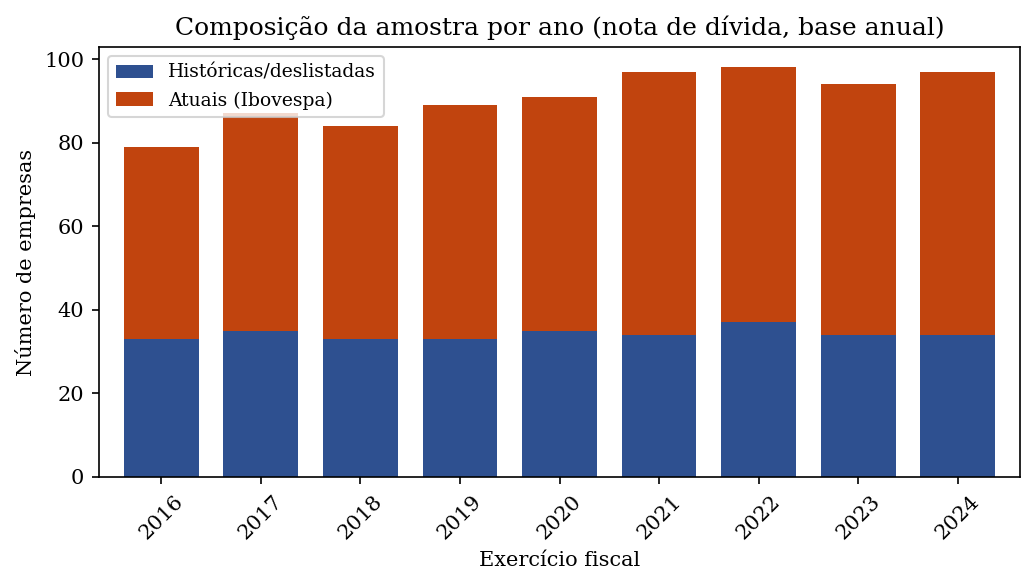
\includegraphics[width=0.85\textwidth]{figures/sample_composition.png}
    \caption{Composição da amostra por exercício fiscal}
    \label{fig:composicao}
    \vspace{0.2cm}

    {\footnotesize Fonte: elaborada pelo autor. Total: 335 pares empresa-ano de empresas atuais e 192 de empresas históricas/deslistadas (amostra de extração confiável, Seção~\ref{sec:confiabilidade}).}
\end{figure}

\section{Fontes de dados}
\label{sec:fontes}

Cinco fontes de texto e três fontes de dados estruturados foram combinadas nesta dissertação, todas descritas a seguir.

\textbf{Texto (variável independente).} As cinco operacionalizações de mudança textual (Seção~\ref{sec:medida}) vêm de dois sistemas de arquivamento da CVM:
\begin{itemize}
    \item \textit{DFP} (Demonstrações Financeiras Padronizadas, anual): fonte da nota de dívida isolada (base anual) e do conjunto completo de notas explicativas.
    \item \textit{ITR} (Informações Trimestrais): fonte da nota de dívida isolada em base trimestral, usada como checagem exploratória de robustez de frequência.
    \item \textit{Formulário de Referência (FRE)}: fonte tanto do Relatório da Administração quanto da seção de Fatores de Risco (item 4.1), um tipo de arquivamento da CVM inteiramente diferente do DFP/ITR, com sua própria estrutura de pacote e, no caso de arquivamentos anteriores a 2021, um formato legado que exigiu um segundo pipeline de extração.
\end{itemize}

\textbf{Dados estruturados (variáveis de controle e de resultado).}
\begin{itemize}
    \item \textit{Demonstrações financeiras padronizadas da CVM} (mesmos pacotes DFP acima, mas os arquivos de dados contábeis estruturados, não as notas em texto livre): fonte de tamanho (ativo total, receita líquida), alavancagem, ROA e ROE, e das mudanças contemporâneas de M2 ($\Delta$ROA, $\Delta$alavancagem, $\Delta$dívida).
    \item \textit{Preços de mercado (Bloomberg)}: preços diários de fechamento da ação e do Ibovespa, 2014--2026, fonte do retorno anormal (variável dependente de H1) e do retorno passado (controle).
    \item \textit{Fatores de risco (NEFIN/USP)}: séries diárias dos fatores de mercado, tamanho, valor e momento ($\mathit{MKT}$, $\mathit{SMB}$, $\mathit{HML}$, $\mathit{WML}$) e da taxa livre de risco para o mercado brasileiro \cite{nefin2026}, fonte do modelo de quatro fatores usado para estimar o retorno anormal (Seção~\ref{sec:var_dependente}).
    \item \textit{Preço-sobre-valor-patrimonial e volume negociado (Bloomberg)}: fonte de \textit{book-to-market} (controle de M3) e de liquidez de mercado (razão de iliquidez de Amihud), esta última testada em especificações adicionais fora do núcleo confirmatório M0-M3.
    \item \textit{Consenso de EPS dos analistas (Bloomberg)}: série trimestral de consenso rolante, fonte da variável de revisão usada na análise complementar de H2 (Seção~\ref{sec:h2_metodologia}).
\end{itemize}

Nenhuma dessas fontes estruturadas depende da heurística de localização de seção usada para o texto (Seção~\ref{sec:coleta}): são dados tabulares já padronizados pela CVM ou pela Bloomberg, o que garante cobertura próxima de 100\% nas variáveis de controle.

\section{Confiabilidade da extração e cobertura da aquisição}
\label{sec:confiabilidade}

A confiabilidade da extração e a cobertura da aquisição não são o mesmo problema, e a fonte de texto determina qual dos dois é o principal fator limitante.

Para a nota de dívida isolada, o arquivamento inteiro (o documento completo de notas explicativas) já está disponível na quase totalidade dos casos: o problema é de \textit{localização precisa da seção} dentro de um documento de 30--150 páginas, dependendo de uma heurística baseada em tamanho de fonte e negrito, não de expressão regular simples, pois os mesmos termos-chave aparecem em sumários, corpo do texto e referências cruzadas. Após seis rodadas de aprimoramento, cada uma validada contra casos de controle conhecidos para garantir ausência de regressão, a taxa de extração classificada como confiável atingiu 69,7\% da amostra completa (997 arquivos), partindo de 43,8\% na primeira rodada. Duas ideias adicionais de aprimoramento (detecção de sumário e navegação por referência cruzada, ``ver Nota N'') foram testadas empiricamente e rejeitadas, por baixo retorno (1,4\% de ganho) e alta taxa de falso positivo (apenas 26\% das correspondências corretas), respectivamente.

Nem todo caso classificado como ``não localizado'' representa necessariamente uma falha de extração: é possível que, para uma empresa específica num exercício específico, não exista de fato uma dívida relevante a divulgar.

Para o Relatório da Administração e a seção de Fatores de Risco, o problema é o inverso: uma vez que o arquivamento é obtido, a seção relevante já vem isolada como um anexo PDF dedicado dentro do pacote de envio da CVM (padrão confirmado por leitura de exemplos reais de empresas distintas antes de ser adotado como regra geral, e não assumido a priori), de modo que não há ambiguidade de localização. O fator limitante passa a ser a \textit{cobertura da aquisição}: o Relatório da Administração foi encontrado em 71,2\% dos arquivamentos possíveis (707 de 993); os Fatores de Risco, adquiridos por um pipeline novo que trata tanto o formato moderno quanto um formato legado pré-2021, atingiram 94,4\% de cobertura (923 de 978), consistente ao longo dos dez exercícios do período.

A Figura~\ref{fig:confiabilidade} resume essas duas métricas lado a lado, deliberadamente rotuladas de forma distinta no gráfico, já que não medem a mesma coisa.

\begin{figure}[htbp]
    \centering
    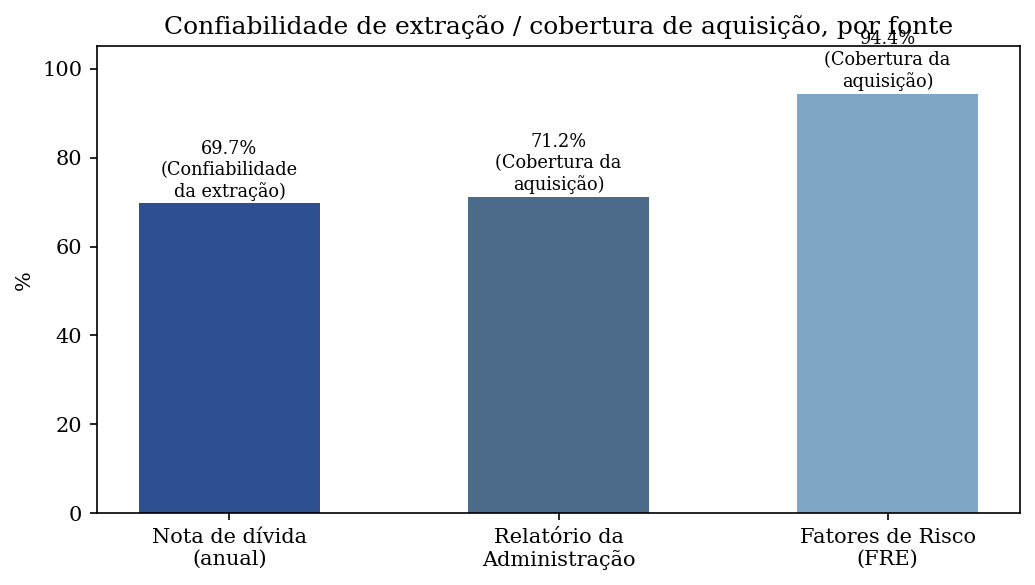
\includegraphics[width=0.8\textwidth]{figures/extraction_reliability.png}
    \caption{Confiabilidade de extração e cobertura de aquisição, por fonte de texto}
    \label{fig:confiabilidade}
    \vspace{0.2cm}

    {\footnotesize Fonte: elaborada pelo autor a partir dos logs de extração/aquisição do projeto.}
\end{figure}

A prática adotada ao longo de todo o projeto foi verificar cada padrão suspeito lendo diretamente uma amostra dos arquivos e casos concretos por trás dele, em vez de confiar apenas na estatística agregada. Foi exatamente essa prática, aplicada em várias rodadas de leitura e teste manual de exemplos, que revelou um problema real de qualidade de dados no cenário de conjunto completo de notas: para uma fração relevante dos arquivos, o anexo capturado era, na verdade, um documento diferente (por exemplo, um release de resultados em vez das demonstrações financeiras). Todos os resultados reportados no Capítulo~\ref{ch:resultados} usam apenas a versão já corrigida para essa contaminação.

\textbf{Regra metodológica: apenas extração confiável para a nota de dívida isolada.} A nota de dívida isolada (base anual e trimestral) é a única fonte de texto sujeita à heurística de localização de seção descrita acima, e portanto a única com uma classificação de confiabilidade (\textit{font\_heading} vs. \textit{regex\_only}) a considerar; as outras três fontes já chegam pré-isoladas, sem essa ambiguidade. A Seção~\ref{sec:poc_validacao} mostra que restringir a amostra a pares com \textit{font\_heading} nos dois anos desloca a distribuição de similaridade para um padrão mais bem comportado (Figura~\ref{fig:similaridade_bruta_confiavel}) sem alterar nenhuma conclusão de H1 ou H2. Diante disso, todos os resultados da nota de dívida isolada reportados a partir daqui -- Tabela~\ref{tab:sample} em diante, Capítulos~\ref{ch:resultados} -- usam exclusivamente essa amostra restrita, não mais o conjunto completo de pares computáveis.

\section{Estatísticas descritivas das variáveis}
\label{sec:estatisticas}

O número de pares ano a ano com similaridade textual calculável varia por fonte de texto, refletindo tanto as diferenças de cobertura da Seção~\ref{sec:confiabilidade} quanto o fato de as fontes mais recentes (conjunto completo de notas, Relatório da Administração, Fatores de Risco) terem sido incorporadas ao corpus em etapas posteriores do projeto (Tabela~\ref{tab:sample}).

\begin{table}[htbp]
    \centering
    \caption{Pares ano a ano por fonte de texto}
    \label{tab:sample}
    \begin{tabular}{@{}llrr@{}}
        \toprule
        \textbf{Fonte de texto} & \textbf{Frequência} & \textbf{Pares} & \textbf{Empresas} \\
        \midrule
        Nota de dívida isolada (total)      & Anual & 816 & 111 \\
        Nota de dívida isolada (confiável)  & Anual & 527 & 99 \\
        Nota de dívida isolada (total)      & Trimestral & 2.572 & 112 \\
        Nota de dívida isolada (confiável)  & Trimestral & 1.496 & 103 \\
        Conjunto completo de notas explicativas & Anual & 487 & 96 \\
        Relatório da Administração & Anual & 562 & 91 \\
        Fatores de Risco (FRE) & Anual & 811 & 110 \\
        \bottomrule
    \end{tabular}
    \\[0.3cm]
    {\footnotesize Fonte: elaborada pelo autor a partir de dados da CVM. ``Total'' = todos os pares com similaridade computável; ``confiável'' = restrito a pares com extração confiável (\textit{font\_heading}) nos dois anos (Seção~\ref{sec:confiabilidade}), a amostra usada nos resultados a partir daqui.}
\end{table}

Dados de mercado (preços diários da ação e do Ibovespa, 2014--2026) cobrem a totalidade das 66 empresas atuais. Dados de consenso de EPS dos analistas (Bloomberg), usados na análise complementar de H2, cobrem 64 das 66 empresas atuais e 27 das 45 históricas.

A nota de dívida isolada em base anual é o objeto central desta dissertação (H1 e H2, Seção~\ref{sec:hipoteses}); as outras quatro fontes de texto entram apenas como critério de comparação metodológica (Seção~\ref{sec:medida}), não como parte do teste das hipóteses. A Figura~\ref{fig:similaridade} compara a distribuição da similaridade de cosseno entre as cinco fontes. Um padrão salta aos olhos e é relevante para a leitura dos resultados do Capítulo~\ref{ch:resultados}: as fontes de documento inteiro ou pré-isolado por seção fixa (conjunto completo de notas, Fatores de Risco) concentram-se muito mais perto de 1 (mediana de 0,95 em ambas) do que a nota de dívida isolada (mediana de 0,83 na base anual, já sobre a amostra de extração confiável). Ou seja, mesmo restrita à extração mais confiável, o recorte estreito da nota específica de dívida ainda captura mais mudança textual ano a ano do que o documento inteiro ou uma seção-padrão como Fatores de Risco, nos quais boilerplate estrutural dilui a mudança relativa -- uma diferença menor do que a observada sobre a amostra completa, mas na mesma direção.

\begin{figure}[htbp]
    \centering
    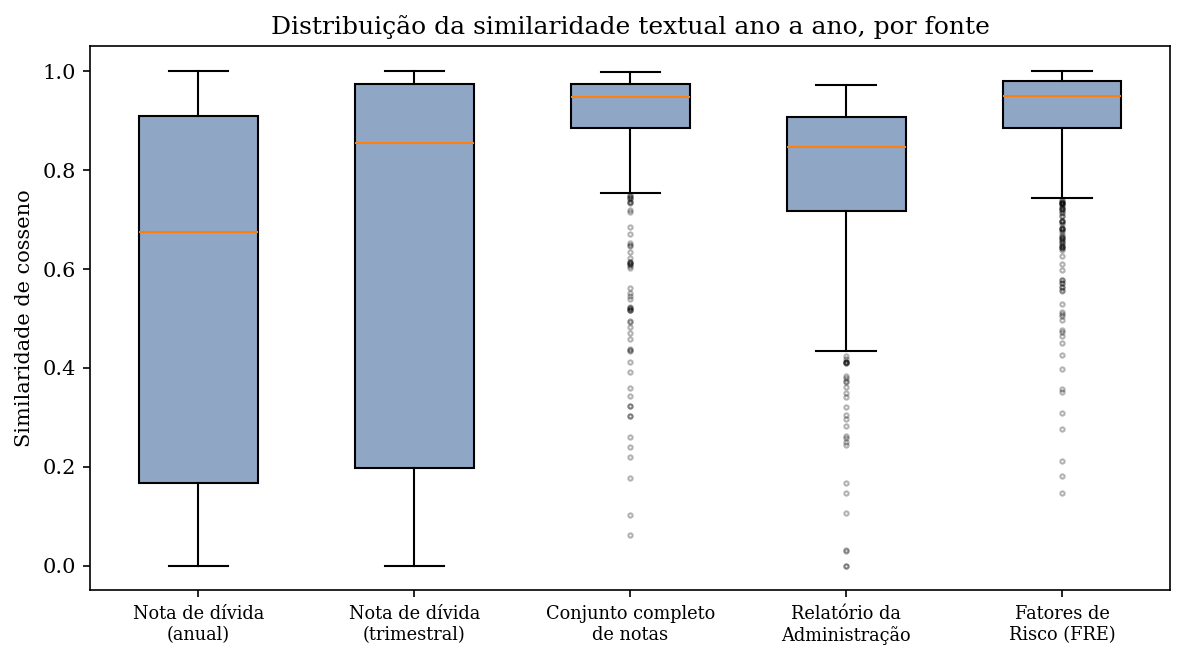
\includegraphics[width=0.85\textwidth]{figures/similarity_by_source.png}
    \caption{Distribuição da similaridade textual ano a ano, por fonte}
    \label{fig:similaridade}
    \vspace{0.2cm}

    {\footnotesize Fonte: elaborada pelo autor. Caixas: 1º-3º quartil; linha central: mediana; pontos: valores atípicos.}
\end{figure}

A Figura~\ref{fig:retorno} mostra a distribuição do retorno anormal (variável dependente de H1, nota de dívida anual, $n=450$ pares). É um subconjunto dos 527 pares com similaridade confiável da Tabela~\ref{tab:sample}: calcular o retorno anormal exige, adicionalmente, um ticker negociável e preço de mercado disponível no período, o que 77 pares não têm (majoritariamente empresas históricas que saíram definitivamente do mercado, Seção~\ref{sec:amostra}). A distribuição é aproximadamente simétrica em torno de uma mediana ligeiramente negativa ($-6{,}7\%$), sem assimetria extrema que por si só explicaria a ausência de significância reportada no Capítulo~\ref{ch:resultados}. Um retorno anormal médio negativo é esperado em um mercado emergente com Ibovespa como referência em períodos de estresse macroeconômico (2015--2016, 2020), e não indica um problema de construção da variável.

\begin{figure}[htbp]
    \centering
    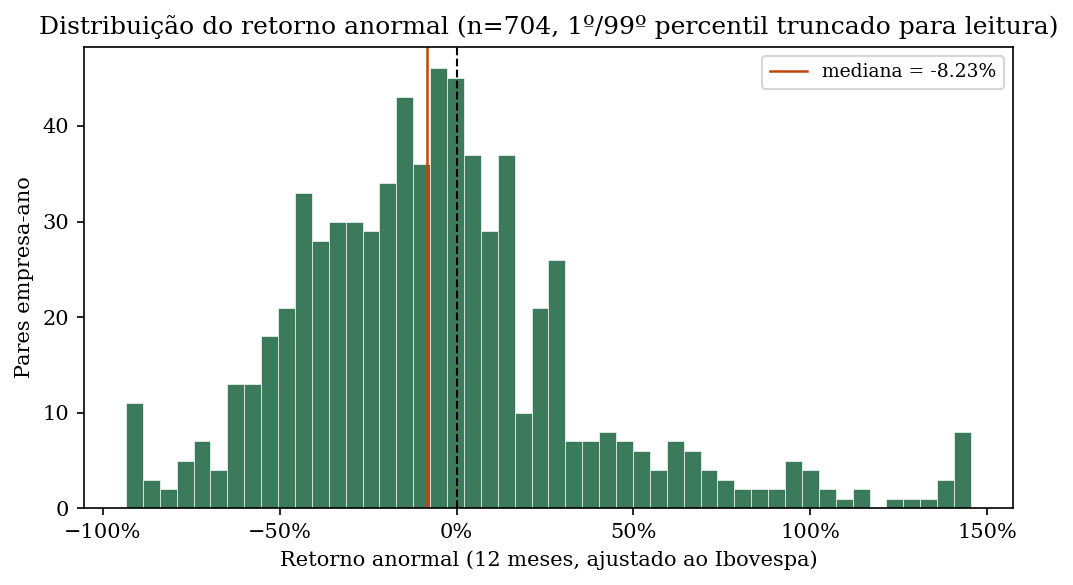
\includegraphics[width=0.8\textwidth]{figures/abnormal_return_dist.png}
    \caption{Distribuição do retorno anormal (nota de dívida, base anual)}
    \label{fig:retorno}
    \vspace{0.2cm}

    {\footnotesize Fonte: elaborada pelo autor a partir de preços da Bloomberg. Percentis 1 e 99 truncados para legibilidade; estatísticas calculadas sobre a amostra de extração confiável.}
\end{figure}

As Figuras~\ref{fig:controles}, \ref{fig:controles_m2} e \ref{fig:controles_m3} mostram a distribuição das nove variáveis de controle da grade M0-M3 (Seção~\ref{sec:controles}), uma figura por bloco: a Figura~\ref{fig:controles} cobre os quatro fundamentos de nível que entram em M1 (tamanho, ROA, alavancagem, momento), sobre as 992 observações empresa-ano com dados contábeis estruturados disponíveis -- um exercício fiscal individual por observação, e não um par ano a ano como nas contagens da Tabela~\ref{tab:sample}, o que explica o número maior; a Figura~\ref{fig:controles_m2} cobre as três mudanças contemporâneas de M2 ($\Delta$ROA, $\Delta$Alavancagem, $\Delta$Dívida); e a Figura~\ref{fig:controles_m3} cobre as duas variáveis de risco/retorno esperado de M3 (\textit{book-to-market} e volatilidade), ambas sobre a amostra da nota de dívida anual (extração confiável). O logaritmo do ativo total tem distribuição aproximadamente normal, como esperado; alavancagem concentra-se abaixo de 1, com uma cauda de poucas empresas em dificuldade financeira severa (passivo superior ao ativo); ROA concentra-se perto de zero com cauda esquerda mais longa (empresas com prejuízo); e o retorno passado tem assimetria positiva característica de retornos de ações.

\begin{figure}[htbp]
    \centering
    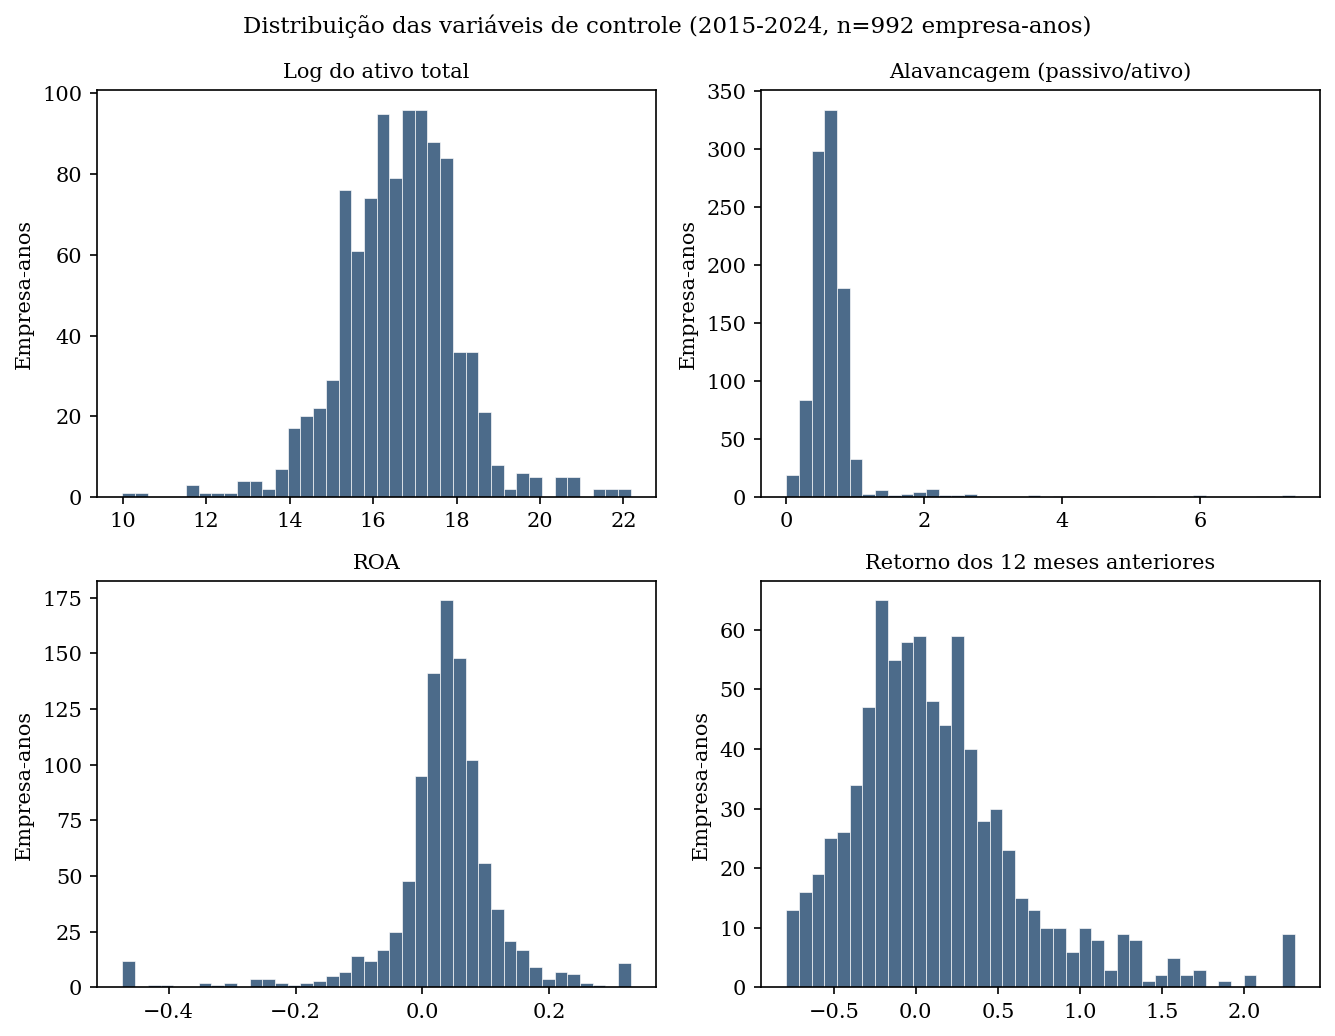
\includegraphics[width=0.85\textwidth]{figures/control_variables.png}
    \caption{Distribuição dos controles de nível (M1)}
    \label{fig:controles}
    \vspace{0.2cm}

    {\footnotesize Fonte: elaborada pelo autor a partir de dados contábeis estruturados da CVM. ROA e retorno passado truncados nos percentis 1/99 para legibilidade.}
\end{figure}

As três mudanças de M2 concentram-se perto de zero, como esperado para uma variação ano a ano em empresas maduras, com caudas moderadas nos dois sentidos (empresas em reestruturação financeira mais acentuada).

\begin{figure}[htbp]
    \centering
    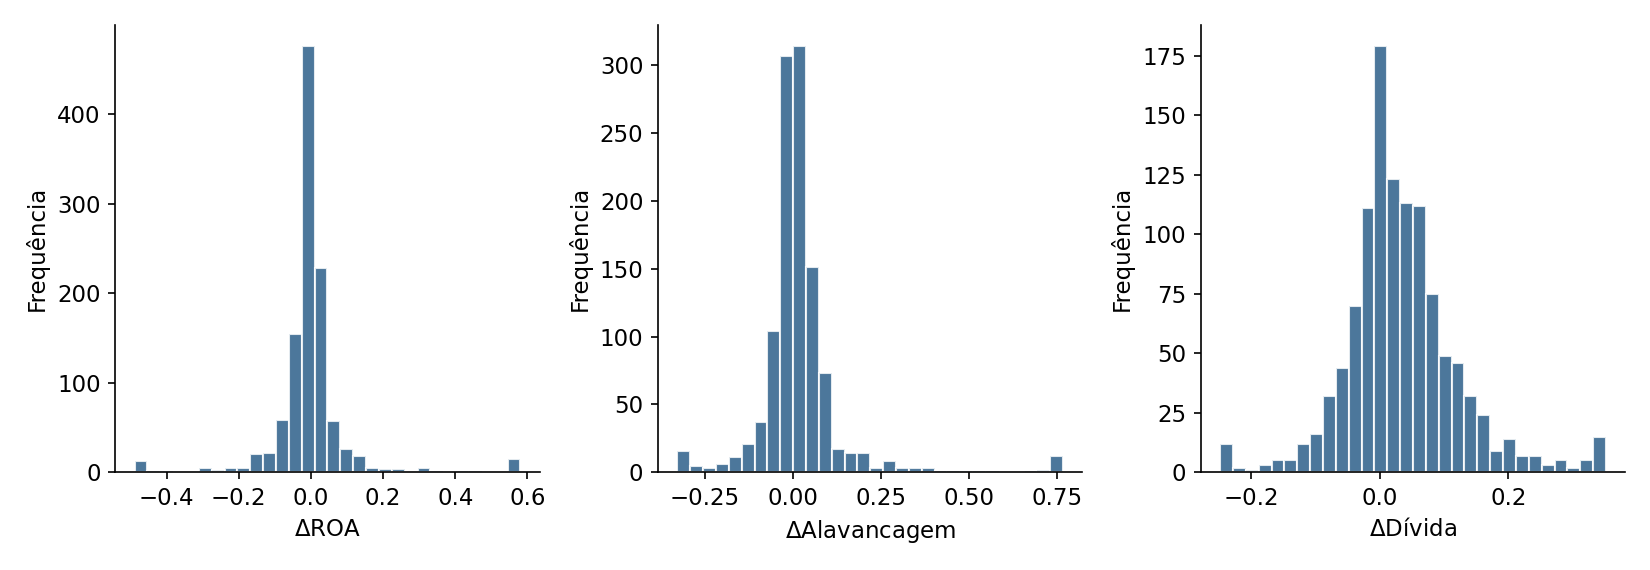
\includegraphics[width=0.95\textwidth]{figures/m2_controls.png}
    \caption{Distribuição dos controles de M2}
    \label{fig:controles_m2}
    \vspace{0.2cm}

    {\footnotesize Fonte: elaborada pelo autor a partir de dados contábeis estruturados da CVM. Percentis 1/99 truncados para legibilidade.}
\end{figure}

O \textit{book-to-market} de M3 tem a assimetria positiva característica dessa variável (poucas empresas negociando muito abaixo do valor patrimonial, a maioria acima), consistente com o que a literatura reporta para outros mercados \cite{famafrench1992}. A volatilidade de M3 concentra-se entre 1,5\% e 3,5\% de desvio-padrão diário, com uma cauda de empresas mais voláteis -- tipicamente aquelas atravessando dificuldade financeira ou operando em setores mais cíclicos no período.

\begin{figure}[htbp]
    \centering
    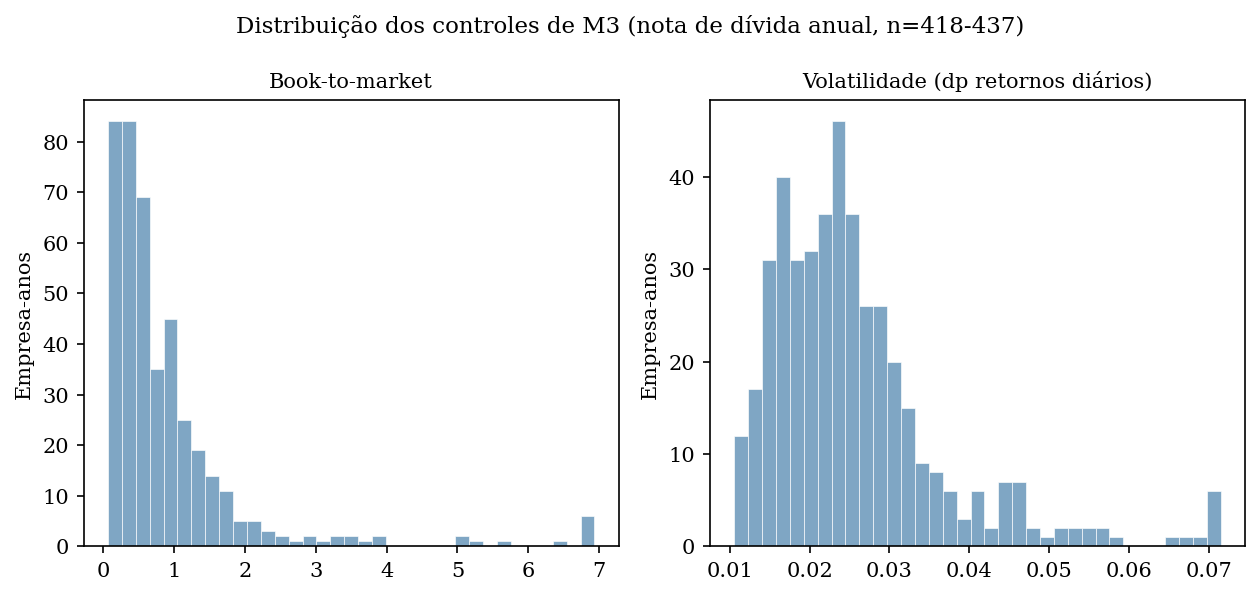
\includegraphics[width=0.75\textwidth]{figures/m3_controls.png}
    \caption{Distribuição dos controles de M3}
    \label{fig:controles_m3}
    \vspace{0.2cm}

    {\footnotesize Fonte: elaborada pelo autor a partir de preços/indicadores de mercado da Bloomberg. Percentis 1/99 truncados para legibilidade.}
\end{figure}

A cobertura é alta nas cinco variáveis de M2/M3: 436 de 437 pares (99,8\%) para as três mudanças contemporâneas e para a volatilidade, e 423 de 437 (96,8\%) para \textit{book-to-market}, cuja pequena lacuna reflete casos sem cotação de preço-sobre-valor-patrimonial disponível na data de referência.

\chapter{Resultados}
\label{ch:resultados}

Este capítulo reporta os resultados obtidos até o momento deste Exame de Qualificação. Os resultados são preliminares no sentido definido pelo curso (mais de 50\% do trabalho está concluído), mas o núcleo empírico já reflete um teste amplo e reprodutível: duas hipóteses (H1 e H2), cinco fontes de texto e a grade M0-M3 de rigor crescente (Seção~\ref{sec:controles}). Todo código, dado intermediário e log de execução referenciados aqui está versionado no repositório do projeto. A descrição da amostra, das fontes de dados e das estatísticas descritivas está no Capítulo~\ref{ch:dados}.

\section{Validação exploratória da medida de mudança textual}
\label{sec:poc_validacao}

Antes dos testes confirmatórios de H1 e H2 (Seções~\ref{sec:h1_resultados}--\ref{sec:h2_resultados}), uma fase exploratória extensa e iterativa verificou se a similaridade TF-IDF aplicada à nota de dívida captura de fato conteúdo textual real, e não apenas ruído de extração. Essa validação não é, em si, um teste de hipótese; é o alicerce que dá suporte à leitura dos resultados nulos das seções seguintes como uma resposta genuína sobre previsibilidade de retorno.

\textbf{Confiabilidade de extração ao longo das rodadas.} A Figura~\ref{fig:trajetoria_extracao} mostra a evolução da taxa de extração confiável (\textit{font\_heading}) sobre o corpus anual completo (997 arquivamentos), rodada a rodada. A rodada 4 estabeleceu a linha de base em 43,8\%; quatro aprimoramentos cumulativos, cada um motivado pela inspeção direta de casos reais de falha e validado contra controles já funcionais para garantir ausência de regressão, elevaram essa taxa para 69,7\%. O maior ganho isolado veio do reconhecimento de títulos em negrito do mesmo tamanho da fonte do corpo do texto (não apenas maiores), que resolveu sozinho 22 empresas que tinham taxa de extração confiável de 0\% em todos os anos verificados. O último aprimoramento reconheceu títulos igualmente sem caixa alta e sem numeração (por exemplo, ``Debêntures'' ou ``Empréstimos e financiamentos'' isolados), desde que compostos apenas pelas próprias palavras-chave da dívida; essa regra exigiu, por sua vez, três salvaguardas específicas contra falsos positivos encontrados por inspeção direta (uma subseção com fonte maior que a própria nota-mãe vencendo por tamanho; fragmentos de frase quebrada linha a linha, reconhecíveis por nunca começarem com letra minúscula; e um parágrafo de política contábil genérica vencendo a nota real por empate de pureza, resolvido priorizando um candidato ancorado por número de nota isolado quando existe) antes de ser aceita como confiável.

\begin{figure}[htbp]
    \centering
    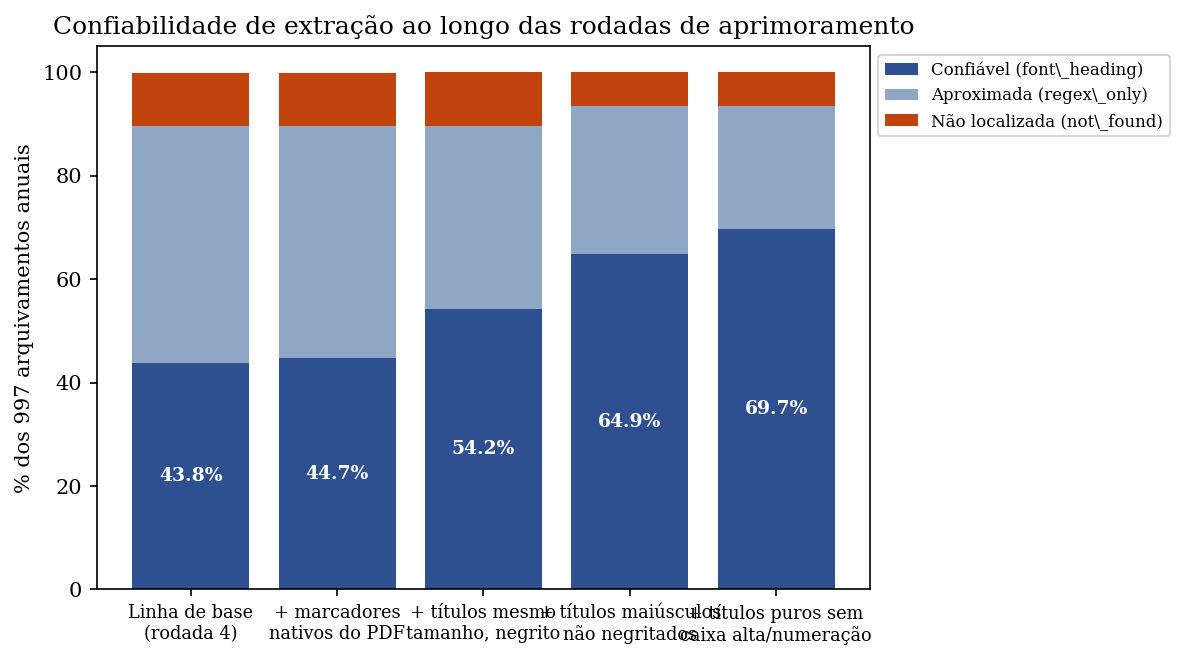
\includegraphics[width=0.85\textwidth]{figures/extraction_hardening_trajectory.png}
    \caption{Confiabilidade de extração ao longo das rodadas de aprimoramento}
    \label{fig:trajetoria_extracao}
    \vspace{0.2cm}

    {\footnotesize Fonte: elaborada pelo autor a partir dos logs de extração do projeto (corpus anual completo, 997 arquivamentos).}
\end{figure}

\textbf{A similaridade se comporta melhor exatamente onde a extração é confiável.} A Figura~\ref{fig:similaridade_bruta_confiavel} compara a distribuição de similaridade sobre todos os pares extraídos com a distribuição restrita aos pares em que ambos os anos tiveram extração confiável. Restringir à extração confiável desloca a média de 0,56 para 0,70 e a mediana de 0,67 para 0,83, e reduz a concentração anômala de escores próximos de 0 e exatamente 1 que caracteriza os casos de falha de extração conhecidos (ver adiante). Esse é o padrão esperado se a medida estiver de fato lendo o texto da nota; não seria o padrão esperado se a variação observada fosse puramente ruído de extração. É essa evidência, junto com a ausência de qualquer mudança nas conclusões de H1 e H2 ao aplicar a restrição (Seção~\ref{sec:h1_resultados}), que motiva adotar a extração confiável como a amostra padrão da nota de dívida isolada em todo o restante do trabalho (Seção~\ref{sec:confiabilidade}), em vez de mantê-la apenas como um teste de robustez à parte.

\begin{figure}[htbp]
    \centering
    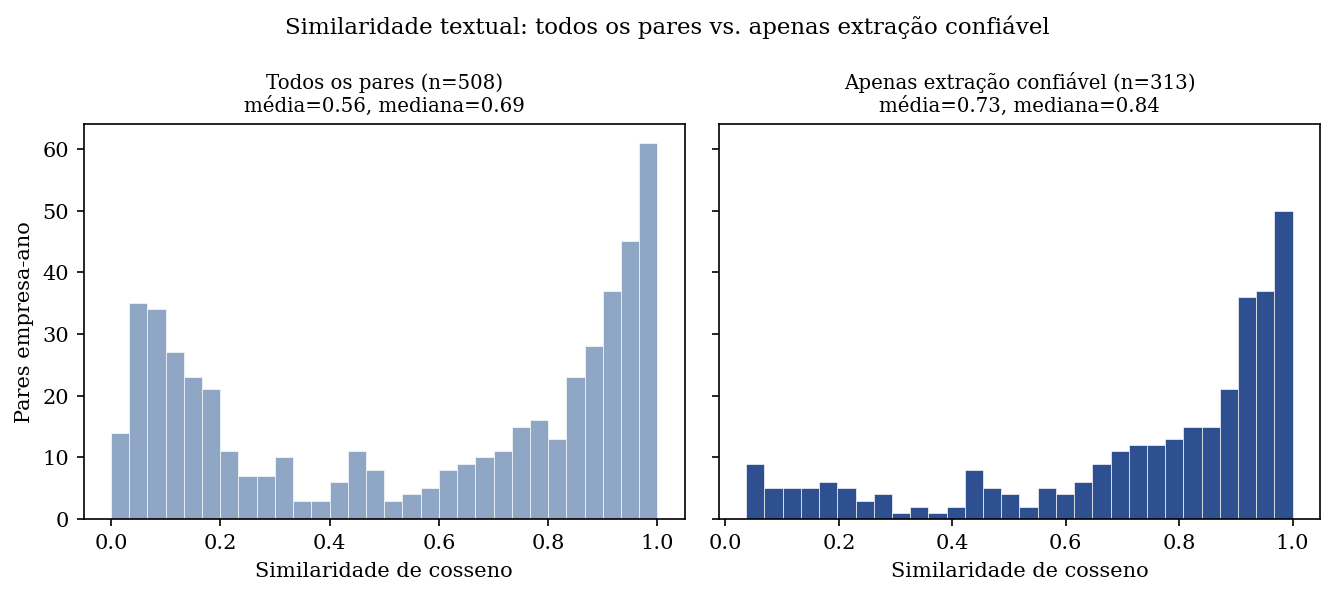
\includegraphics[width=0.9\textwidth]{figures/similarity_raw_vs_reliable.png}
    \caption{Distribuição da similaridade textual: todos os pares vs. apenas extração confiável}
    \label{fig:similaridade_bruta_confiavel}
    \vspace{0.2cm}

    {\footnotesize Fonte: elaborada pelo autor a partir de \textit{delisted\_similarity\_results.csv} (corpus anual completo, 111 empresas).}
\end{figure}

\textbf{Dois casos concretos.} WEG (2015$\to$2016, similaridade 0,9902) é um exemplo de similaridade genuinamente alta: a estrutura da nota é praticamente idêntica entre os dois anos, apenas valores e data mudam, o padrão de ``boilerplate atualizado com novos números''. Já a Yduqs (2017$\to$2018 e 2018$\to$2019, similaridade exatamente 1,0000 nos dois pares) é um exemplo de falha de extração: o localizador capturou por engano, nesses três exercícios, o mesmo parágrafo genérico de política contábil em vez da nota real. Todo escore degenerado (exatamente 0 ou 1) inspecionado neste projeto rastreou até uma falha de extração conhecida, não até uma falha da própria medida de similaridade.

\textbf{Checagem exploratória de plausibilidade econômica: saída do Ibovespa.} Como uma verificação adicional de que a medida capta algo economicamente sensato antes dos testes formais, comparou-se a similaridade textual de empresas que saíram do Ibovespa em algum momento do período (por delistagem, fusão ou reestruturação societária) com a das empresas que permaneceram, sobre pares com extração confiável em ambos os anos (Figura~\ref{fig:sobrevivencia}). A direção é a esperada pela lógica teórica do projeto (empresas em dificuldade tendem a mudar mais o texto da nota e também a sair do índice): mediana de 0,832 entre as que saíram contra 0,829 entre as que permaneceram. Sobre o universo completo e não enviesado (192 pares de empresas que saíram, 335 de empresas que permaneceram), essa diferença não atinge significância convencional (Mann-Whitney unilateral, $p=0{,}359$), um resultado consistente com a checagem de deslistamento formal reportada na Seção~\ref{sec:robustez} para a nota de dívida isolada. O valor desta checagem exploratória não está em produzir um achado citável, mas em mostrar que a direção do efeito é sempre a esperada teoricamente, mesmo quando não significativa, o que pesa contra a hipótese de que a medida é apenas ruído aleatório.

\begin{figure}[htbp]
    \centering
    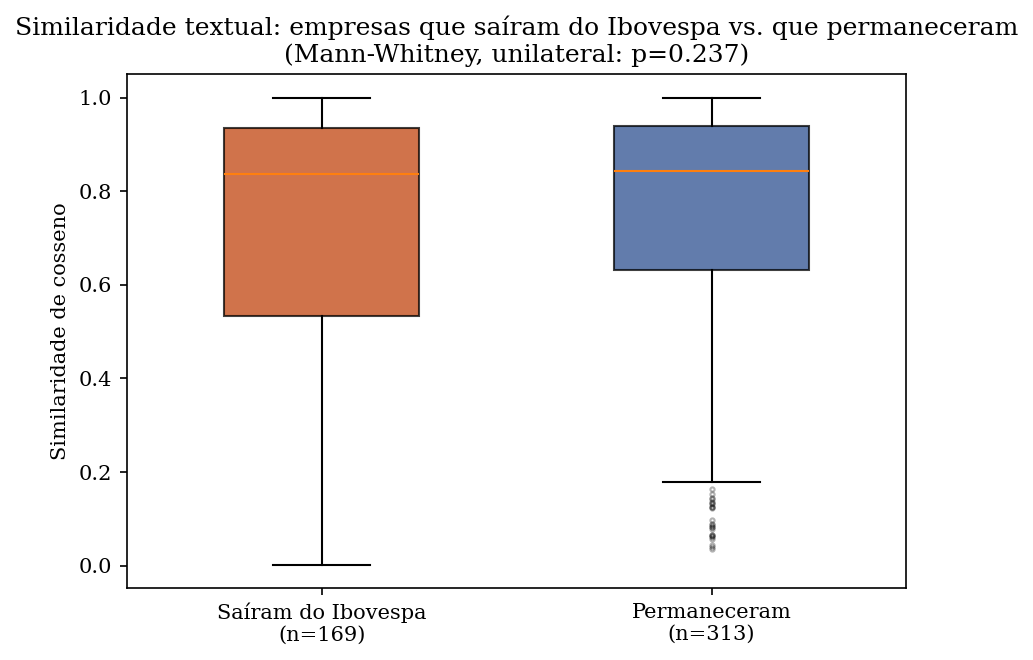
\includegraphics[width=0.7\textwidth]{figures/survivorship_boxplot.png}
    \caption{Similaridade textual: empresas que saíram do Ibovespa vs. que permaneceram}
    \label{fig:sobrevivencia}
    \vspace{0.2cm}

    {\footnotesize Fonte: elaborada pelo autor a partir de \textit{delisted\_similarity\_results.csv} (POC, pares com extração confiável em ambos os anos).}
\end{figure}

Em conjunto, essas três verificações (evolução da confiabilidade de extração, comportamento da distribuição de similaridade e plausibilidade econômica direcional) sustentam a leitura de que o pipeline de dados capta um sinal textual real e interpretável. É sobre essa base que os testes formais de H1 e H2, a seguir, devem ser lidos: o resultado nulo reportado nas próximas seções reflete ausência de evidência estatística suficiente de previsibilidade de retorno e de revisão de consenso, no desenho, na amostra e no poder estatístico disponíveis -- não uma prova de que essa previsibilidade não existe.

\section{Resultados do modelo principal (H1)}
\label{sec:h1_resultados}

A Tabela~\ref{tab:h1} reporta o p-valor do coeficiente de TextChange sobre o BHAR ajustado (Seção~\ref{sec:var_dependente}), para cada fonte de texto, ao longo da grade M0-M3 (Seção~\ref{sec:controles}): M0 (TextChange isolado, com efeitos fixos de empresa e ano), M1 (mais tamanho, ROA, alavancagem e momento), M2 (mais as mudanças contemporâneas de ROA, alavancagem e dívida -- especificação principal) e M3 (mais \textit{book-to-market} e volatilidade).

\begin{table}[htbp]
    \centering
    \caption{Resultados do modelo principal (H1) por fonte de texto, grade M0-M3}
    \label{tab:h1}
    \small
    \begin{tabular}{@{}lrrrrr@{}}
        \toprule
        \textbf{Fonte de texto} & \textbf{n (M3)} & \textbf{M0} & \textbf{M1} & \textbf{M2*} & \textbf{M3} \\
        \midrule
        Nota de dívida (anual)       & 418 & 0,211 & 0,265 & 0,268 & 0,421 \\
        Nota de dívida (trimestral)  & 437 & 0,563 & 0,506 & 0,286 & 0,390 \\
        Conjunto completo de notas   & 404 & 0,424 & 0,683 & 0,631 & 0,611 \\
        Relatório da Administração   & 462 & 0,781 & 0,908 & 0,928 & 0,949 \\
        Fatores de Risco (FRE)       & 650 & 0,420 & 0,355 & 0,359 & 0,197 \\
        \bottomrule
    \end{tabular}
    \\[0.3cm]
    {\footnotesize Fonte: elaborada pelo autor. Valores são p-valores do coeficiente de TextChange, erros-padrão agrupados por empresa em todos os modelos (M0-M3 incluem efeitos fixos de empresa e ano). *M2 é a especificação principal (Seção~\ref{sec:controles}). Nota de dívida (anual e trimestral): amostra restrita a pares com extração confiável (Seção~\ref{sec:confiabilidade}). Coeficientes, erros-padrão e intervalos de confiança completos para todas as células estão na Tabela~\ref{tab:h1_m2_detalhe} e em \textit{m0\_m3\_all\_sources\_results.csv}.}
\end{table}

Nenhuma fonte de texto mostra associação significativa com o retorno anormal em nenhum estágio da grade. É um resultado nulo consistente, não sensível à especificação de controles escolhida -- e, notavelmente, mais nulo do que sob a especificação exploratória anterior: o Relatório da Administração, a única fonte que já havia mostrado algum sinal (retorno ajustado ao mercado, regressão agrupada com controles, $p=0{,}031$), agora não se aproxima da significância em nenhum M ($p \geq 0{,}78$ em todos). A Tabela~\ref{tab:h1_m2_detalhe} detalha o coeficiente, o erro-padrão e o intervalo de confiança de 95\% de cada modelo e cada fonte.

\begin{table}[htbp]
    \centering
    \caption{H1, grade M0-M3 completa: coeficiente, erro-padrão e IC 95\% por fonte de texto e modelo}
    \label{tab:h1_m2_detalhe}
    \small
    \begin{tabular}{@{}llrrrr@{}}
        \toprule
        \textbf{Fonte de texto} & \textbf{M} & \textbf{n} & \textbf{$\hat\beta$ (EP)} & \textbf{IC 95\%} & \textbf{p} \\
        \midrule
        Nota de dívida (anual)      & M0 & 437 & 0,175 (0,140) & [$-$0,100; 0,449] & 0,211 \\
                                     & M1 & 432 & 0,117 (0,105) & [$-$0,089; 0,324] & 0,265 \\
                                     & M2* & 432 & 0,106 (0,095) & [$-$0,082; 0,293] & 0,268 \\
                                     & M3 & 418 & 0,078 (0,097) & [$-$0,113; 0,270] & 0,421 \\
        Nota de dívida (trimestral) & M0 & 504 & $-$0,015 (0,027) & [$-$0,068; 0,037] & 0,563 \\
                                     & M1 & 501 & $-$0,019 (0,028) & [$-$0,073; 0,036] & 0,506 \\
                                     & M2* & 456 & $-$0,031 (0,029) & [$-$0,088; 0,026] & 0,286 \\
                                     & M3 & 437 & $-$0,025 (0,029) & [$-$0,082; 0,032] & 0,390 \\
        Conjunto completo de notas  & M0 & 416 & $-$0,185 (0,231) & [$-$0,640; 0,270] & 0,424 \\
                                     & M1 & 411 & $-$0,068 (0,167) & [$-$0,396; 0,260] & 0,683 \\
                                     & M2* & 411 & $-$0,078 (0,163) & [$-$0,400; 0,243] & 0,631 \\
                                     & M3 & 404 & $-$0,085 (0,166) & [$-$0,411; 0,242] & 0,611 \\
        Relatório da Administração  & M0 & 489 & 0,076 (0,275) & [$-$0,465; 0,617] & 0,781 \\
                                     & M1 & 484 & 0,028 (0,241) & [$-$0,446; 0,502] & 0,908 \\
                                     & M2* & 484 & 0,022 (0,244) & [$-$0,457; 0,502] & 0,928 \\
                                     & M3 & 462 & $-$0,016 (0,251) & [$-$0,509; 0,477] & 0,949 \\
        Fatores de Risco (FRE)      & M0 & 677 & 0,184 (0,228) & [$-$0,264; 0,631] & 0,420 \\
                                     & M1 & 672 & 0,198 (0,214) & [$-$0,222; 0,619] & 0,355 \\
                                     & M2* & 672 & 0,211 (0,230) & [$-$0,241; 0,664] & 0,359 \\
                                     & M3 & 650 & 0,298 (0,231) & [$-$0,155; 0,752] & 0,197 \\
        \bottomrule
    \end{tabular}
    \\[0.3cm]
    {\footnotesize Fonte: elaborada pelo autor. EP = erro-padrão agrupado por empresa. *M2 é a especificação principal. Todos os intervalos de confiança contêm zero, em todo modelo e toda fonte. Nota de dívida (anual e trimestral): amostra restrita a pares com extração confiável (Seção~\ref{sec:confiabilidade}).}
\end{table}

Um padrão nos coeficientes (não apenas nos p-valores) vale registrar: o sinal de $\hat\beta$ é positivo -- mais mudança textual associada a mais retorno anormal futuro -- na nota de dívida anual e nos Fatores de Risco em todo M0-M3, e na nota trimestral e no conjunto completo de notas é negativo em todo M0-M3. Nenhum dos dois padrões é significativo, e o próprio sinal do efeito não é interpretado como achado (Seção~\ref{sec:leitura_beta}, ``Como ler $\beta$''); mas a inconsistência de sinal entre fontes que deveriam, em princípio, captar o mesmo mecanismo é ela própria uma informação: pesa contra uma leitura de que existe um efeito real pequeno e apenas não detectado por falta de poder estatístico, e a favor de que o que se observa em cada fonte, nesses coeficientes de magnitude pequena e não significativa, é majoritariamente ruído amostral.

O padrão de resultados por fonte de texto também não é aleatório em relação à teoria. \citeonline{cohen2020} e \citeonline{amelzadeh2016} documentam, dentro de suas próprias amostras, que o efeito de mudança textual sobre retorno futuro se concentra em texto de alta discricionariedade gerencial (Risk Factors, MD\&A) e é mais fraco em texto formulaico e auditado, como notas explicativas contábeis. O Relatório da Administração, o equivalente brasileiro ao MD\&A, e a seção de Fatores de Risco, adquirida especificamente para testar essa previsão da literatura, são as fontes de maior discricionariedade narrativa entre as testadas -- e, ainda assim, nenhuma mostra associação significativa em nenhum estágio da grade M0-M3, o que pesa contra uma leitura simples de ``falta a fonte de texto certa''.

\section{Testes de robustez}
\label{sec:robustez}

Numa etapa exploratória anterior deste trabalho, com o retorno ajustado ao mercado sem beta (Seção~\ref{sec:var_dependente}) e um conjunto de controles escolhido \textit{a posteriori}, o Relatório da Administração chegou a mostrar um coeficiente significativo numa única especificação (regressão agrupada com controles, $p=0{,}031$). Esse indício foi submetido a uma bateria extensa de verificação -- perturbação da amostra (winsorização, remoção de extremos, exclusão empresa a empresa, correlação de postos), um teste de portfólio calendário independente e efeitos fixos de empresa e ano -- por precaução, já que duas outras vezes neste projeto uma associação inicialmente significativa ($p<0{,}01$) revelou-se, após verificação, um artefato de coleta de dados. O indício não sobreviveu a efeitos fixos ($p=0{,}478$ sob a especificação exploratória) nem ao teste de portfólio (melhor caso $p=0{,}276$), e não reaparece em nenhuma célula da grade M0-M3 sob a especificação definitiva de retorno anormal (Tabela~\ref{tab:h1}, $p \geq 0{,}78$ em todo M para o Relatório da Administração). O detalhamento completo da bateria de perturbação está preservado no histórico de versões do repositório do projeto, não reproduzido aqui por não ser mais relevante para a leitura dos resultados finais.

\textbf{Checagem de associação com saída do índice.} Testou-se, para cada fonte de texto, se TextChange está associado à saída subsequente da empresa do Ibovespa (Tabela~\ref{tab:delisting}).

\begin{table}[htbp]
    \centering
    \caption{Associação entre TextChange e saída do índice, por fonte de texto}
    \label{tab:delisting}
    \begin{tabular}{@{}lrr@{}}
        \toprule
        \textbf{Fonte de texto} & \textbf{Sem controles} & \textbf{Modelo principal (M2)} \\
        \midrule
        Nota de dívida (anual)      & 0,649 & 0,754 \\
        Conjunto completo de notas  & 0,086 & 0,370 \\
        Relatório da Administração  & \textbf{0,033} & 0,127 \\
        \bottomrule
    \end{tabular}
    \\[0.3cm]
    {\footnotesize Nota de dívida (anual): amostra restrita a pares com extração confiável (Seção~\ref{sec:confiabilidade}).}
\end{table}

O Relatório da Administração é, novamente, a única fonte com algum sinal sem controles, mas não sobrevive à adição dos controles de M2 (tamanho, ROA, alavancagem, momento e as três mudanças contemporâneas). Um teste de efeitos fixos não foi aplicado a essa checagem especificamente: a condição de deslistamento é constante dentro de cada empresa, e a transformação de efeitos fixos elimina exatamente a variação que se quer explicar. Estimar o modelo mesmo assim produz um coeficiente de ordem $10^{-17}$ (essencialmente zero de máquina) acompanhado de um p-valor de 0,0057, que pareceria altamente significativo se lido sem esse cuidado. Esse é um exemplo concreto de um teste mal especificado, identificado e descartado antes de ser reportado como resultado.

\textbf{Achado adicional: Fatores de Risco e saída do índice, com desenho corrigido.} A checagem de deslistamento é, por natureza, uma pergunta no nível da empresa, não no nível do par ano a ano: o desenho tecnicamente correto é uma única observação por empresa. Construiu-se uma variável de TextChange média por empresa, com os controles de M2 também agregados por empresa (média entre pares), e estimou-se uma regressão puramente transversal (Tabela~\ref{tab:riskfactors}).

\begin{table}[htbp]
    \centering
    \caption{Fatores de Risco e saída do índice: desenho transversal}
    \label{tab:riskfactors}
    \begin{tabular}{@{}p{6.5cm}rrr@{}}
        \toprule
        \textbf{Especificação} & \textbf{n} & \textbf{Coef.} & \textbf{p-valor} \\
        \midrule
        Sem controles                              & 94 & $1{,}99$ & \textbf{0,011} \\
        Modelo principal (M2), MQO                  & 94 & $1{,}76$ & \textbf{0,026} \\
        Modelo principal (M2), logit                & 94 & $15{,}71$ & \textbf{0,015} \\
        \bottomrule
    \end{tabular}
    \\[0.3cm]
    {\footnotesize $n=94$, não 110: 16 empresas perdem cobertura ao exigir os sete controles de M2 (sobretudo $\Delta$Dívida, que depende de dois exercícios consecutivos de dados contábeis).}
\end{table}

O coeficiente é positivo e consistente com a direção esperada: maior TextChange médio (mais mudança textual) associa-se a maior probabilidade de saída do índice. Diferentemente do achado do Relatório da Administração, este desenho não sofre do problema de observações repetidas em primeiro lugar, de modo que não há um teste mais rigoroso disponível capaz de invalidá-lo pela mesma via. O resultado sobrevive à troca do conjunto de controles ad hoc original pelos controles de M2, teoricamente justificados -- um resultado que se mantém sob um conjunto de controles mais rigoroso é mais crível do que um que só aparece sob um conjunto escolhido \textit{a posteriori}. Mas a robustez não é completa: sob os controles de M2, a exclusão de cada empresa individualmente produz um pior caso de $p=0{,}107$, e substituir a média por mediana na agregação por empresa dá $p=0{,}120$ -- ambos acima do limiar de 5\%, diferente do que se observava sob o conjunto de controles antigo (pior caso $p=0{,}078$; mediana $p=0{,}033$). O achado central permanece significativo na especificação principal, mas é mais sensível a essas perturbações do que parecia antes.

Esse é, no conjunto, o achado empírico mais bem sustentado deste projeto até o momento, mas sua interpretação deve ser precisa e sua robustez não deve ser superestimada. Ele diz respeito à validade da medida de mudança textual como sinal de dificuldade da empresa, não à hipótese central H1 de que a mudança textual prevê retorno futuro; essa última permanece nula inclusive para os Fatores de Risco.

\textbf{Comparação direta com o desenho de \citeonline{santoscoelho2018}.} Como verificação adicional, motivada diretamente pela limitação que os próprios autores apontam (Seção~\ref{sec:identificacao}), o modelo de retorno anormal foi reestimado seguindo o desenho metodológico deles o mais de perto possível: efeito único de empresa (sem efeito de ano), escolhido por teste de Hausman a cada especificação (efeitos fixos quando o teste rejeita a hipótese nula de equivalência, efeitos aleatórios caso contrário), com erros-padrão robustos à heterocedasticidade em vez de agrupados por empresa, com TextChange e o BHAR ajustado (Seção~\ref{sec:var_dependente}) no lugar da similaridade e do retorno ajustado ao mercado. A diferença deliberada é o painel: dez exercícios (2015--2024) em vez de três, permitindo que o teste de Hausman discrimine com mais confiança entre as duas abordagens (Tabela~\ref{tab:santoscoelho}).

\begin{table}[htbp]
    \centering
    \caption{Retorno anormal sob o desenho metodológico de Santos e Coelho (2018)}
    \label{tab:santoscoelho}
    \small
    \resizebox{\textwidth}{!}{%
    \begin{tabular}{@{}llrrrrl@{}}
        \toprule
        \textbf{Fonte de texto} & \textbf{Janela} & \textbf{Ef. fixos (2 vias)} & \textbf{FE (só empresa)} & \textbf{RE (só empresa)} & \textbf{Hausman} & \textbf{Escolhido} \\
        \midrule
        Nota de dívida (anual)      & 12m & 0,272 & 0,307 & 0,229 & 0,348 & RE: 0,229 \\
                                     & 18m & 0,104 & 0,071 & 0,192 & 0,469 & RE: 0,192 \\
        Conjunto completo de notas  & 12m & 0,686 & 0,953 & 0,717 & 0,030 & FE: 0,953 \\
                                     & 18m & 0,983 & 0,992 & 0,924 & 0,011 & FE: 0,992 \\
        Relatório da Administração  & 12m & 0,895 & 0,526 & 0,533 & 0,005 & FE: 0,526 \\
                                     & 18m & 0,321 & 0,092 & 0,415 & 0,010 & FE: 0,092 \\
        Fatores de Risco            & 12m & 0,365 & 0,352 & 0,735 & 0,000 & FE: 0,352 \\
                                     & 18m & 0,923 & 0,908 & 0,578 & 0,078 & RE: 0,578 \\
        \bottomrule
    \end{tabular}%
    }
    \\[0.3cm]
    {\footnotesize Fonte: elaborada pelo autor. Valores são p-valores do coeficiente de TextChange, exceto a coluna Hausman (p-valor do teste de especificação) e a última coluna, que reporta o estimador escolhido pela regra de \citeonline{santoscoelho2018} (Hausman rejeita a 5\% $\rightarrow$ efeitos fixos; caso contrário, efeitos aleatórios) e o p-valor correspondente. Nota de dívida (anual): amostra restrita a pares com extração confiável (Seção~\ref{sec:confiabilidade}).}
\end{table}

Nenhuma fonte de texto e nenhuma janela mostra significância em nenhuma das duas versões do desenho, sob nenhum dos dois métodos de agrupamento (Hausman ou dois-vias). O caso mais próximo de significância -- Relatório da Administração aos 18 meses, efeitos fixos apenas de empresa, $p=0{,}092$ -- ainda está longe do limiar convencional.

Esse exercício responde diretamente à limitação que os autores apontam em seu próprio estudo: um painel mais longo, dizem eles, poderia revelar diferenças relevantes entre as abordagens de efeito fixo e aleatório que um painel curto não capta com confiança. Um painel mais de três vezes mais longo (dez exercícios contra três) permite exatamente esse teste com mais poder estatístico, e o resultado, em vez de fortalecer ou reverter o achado nulo, o confirma sob mais uma combinação de modelo, amostra e -- agora -- de especificação de retorno anormal. Isso não invalida a contribuição de \citeonline{santoscoelho2018}, que trata de uma pergunta diferente (valor de mercado corrente, não retorno futuro) com um recorte amostral diferente; mas sugere que, ao menos para a relação entre mudança textual e retorno futuro, a inconclusividade não é um artefato de painel curto nem da escolha de retorno ajustado ao mercado sem beta. Ela persiste mesmo quando essas duas limitações específicas são removidas.

\textbf{TF-IDF sem informação futura.} Como registrado na Seção~\ref{sec:medida}, ajustar o IDF sobre o corpus inteiro (2015--2024) levanta uma preocupação de \textit{look-ahead}: a representação de uma nota antiga é influenciada pela frequência de palavras observada em notas futuras. Para testar diretamente essa preocupação, a similaridade da nota de dívida anual foi recalculada usando IDF em janela expansiva -- um ajuste por exercício corrente, usando apenas documentos disponíveis até aquele exercício, refeito uma vez para cada um dos nove anos de referência (2016--2024) em vez de um único ajuste sobre todo o período. A correlação entre a similaridade original e a recalculada é de $0{,}9993$ (diferença absoluta média de $0{,}006$ em uma escala de 0 a 1), e reestimar H1 (grade M0-M3, BHAR ajustado) sobre a versão sem informação futura não altera nenhuma conclusão ($p=0{,}266$ em M2, contra $p=0{,}268$ na versão original). A preocupação com \textit{look-ahead} é legítima em princípio, mas seu impacto prático nesta amostra é desprezível.

\section{Análise complementar (H2)}
\label{sec:h2_resultados}

Como análise complementar (Seção~\ref{sec:h2_metodologia}), testou-se se TextChange também se associa à revisão do consenso de EPS dos analistas em torno da data de divulgação, seguindo a mesma grade M0-M3 da Seção~\ref{sec:h1_resultados} para as quatro fontes de texto aplicáveis (nota de dívida anual e trimestral já restritas à amostra de extração confiável, Seção~\ref{sec:confiabilidade}). O resultado é um nulo limpo em toda a grade: nenhuma fonte atinge significância a 5\% em nenhum M (Tabela~\ref{tab:h2}); a Tabela~\ref{tab:h2_detalhe} traz o coeficiente, o erro-padrão e o intervalo de confiança de 95\% de cada célula.

\begin{table}[htbp]
    \centering
    \caption{Resultados da análise complementar (H2) por fonte de texto, grade M0-M3}
    \label{tab:h2}
    \small
    \begin{tabular}{@{}lrrrrr@{}}
        \toprule
        \textbf{Fonte de texto} & \textbf{n (M3)} & \textbf{M0} & \textbf{M1} & \textbf{M2*} & \textbf{M3} \\
        \midrule
        Nota de dívida (anual)       & 339 & 0,704 & 0,826 & 0,839 & 0,746 \\
        Nota de dívida (trimestral)  & 378 & 0,365 & 0,346 & 0,314 & 0,268 \\
        Conjunto completo de notas   & 316 & 0,913 & 0,897 & 0,932 & 0,780 \\
        Relatório da Administração   & 386 & 0,629 & 0,972 & 0,735 & 0,631 \\
        \bottomrule
    \end{tabular}
    \\[0.3cm]
    {\footnotesize Fonte: elaborada pelo autor. Valores são p-valores do coeficiente de TextChange, erros-padrão agrupados por empresa. *M2 é a especificação principal. Nota de dívida (anual e trimestral): amostra restrita a pares com extração confiável (Seção~\ref{sec:confiabilidade}). Fatores de Risco não consta: a revisão de consenso não foi construída para essa fonte.}
\end{table}

\begin{table}[htbp]
    \centering
    \caption{H2, grade M0-M3 completa: coeficiente, erro-padrão e IC 95\% por fonte de texto e modelo}
    \label{tab:h2_detalhe}
    \small
    \begin{tabular}{@{}llrrrr@{}}
        \toprule
        \textbf{Fonte de texto} & \textbf{M} & \textbf{n} & \textbf{$\hat\beta$ (EP)} & \textbf{IC 95\%} & \textbf{p} \\
        \midrule
        Nota de dívida (anual)      & M0 & 344 & 0,206 (0,540) & [$-$0,858; 1,270] & 0,704 \\
                                     & M1 & 339 & 0,127 (0,576) & [$-$1,009; 1,262] & 0,826 \\
                                     & M2* & 339 & 0,118 (0,577) & [$-$1,018; 1,254] & 0,839 \\
                                     & M3 & 339 & 0,182 (0,562) & [$-$0,926; 1,290] & 0,746 \\
        Nota de dívida (trimestral) & M0 & 422 & $-$0,841 (0,928) & [$-$2,665; 0,984] & 0,365 \\
                                     & M1 & 414 & $-$0,806 (0,854) & [$-$2,486; 0,875] & 0,346 \\
                                     & M2* & 378 & $-$0,947 (0,937) & [$-$2,792; 0,899] & 0,314 \\
                                     & M3 & 378 & $-$1,061 (0,956) & [$-$2,943; 0,821] & 0,268 \\
        Conjunto completo de notas  & M0 & 323 & 0,080 (0,731) & [$-$1,360; 1,520] & 0,913 \\
                                     & M1 & 316 & $-$0,093 (0,721) & [$-$1,514; 1,327] & 0,897 \\
                                     & M2* & 316 & 0,064 (0,745) & [$-$1,404; 1,532] & 0,932 \\
                                     & M3 & 316 & 0,221 (0,788) & [$-$1,331; 1,772] & 0,780 \\
        Relatório da Administração  & M0 & 391 & $-$0,388 (0,802) & [$-$1,965; 1,189] & 0,629 \\
                                     & M1 & 386 & 0,025 (0,717) & [$-$1,385; 1,435] & 0,972 \\
                                     & M2* & 386 & 0,236 (0,694) & [$-$1,130; 1,601] & 0,735 \\
                                     & M3 & 386 & 0,350 (0,729) & [$-$1,084; 1,784] & 0,631 \\
        \bottomrule
    \end{tabular}
    \\[0.3cm]
    {\footnotesize Fonte: elaborada pelo autor. EP = erro-padrão agrupado por empresa. *M2 é a especificação principal. Todos os intervalos de confiança contêm zero, em todo modelo e toda fonte.}
\end{table}

Uma bateria secundária de testes exploratórios (comparação de tercil de TextChange e uma checagem de deslistamento aplicada à revisão), construída antes da adoção da grade M0-M3 e ainda sobre o conjunto de controles anterior (alavancagem, ROA, retorno passado, sem as mudanças contemporâneas nem \textit{book-to-market}/volatilidade), havia produzido três células com $p<0{,}05$ em 56 testes -- um número próximo do esperado por acaso puro, e nenhuma das três sobreviveu à inspeção (padrão de tercil não monotônico em duas, e a checagem de deslistamento perdendo significância sob agrupamento por empresa na terceira). Essa bateria não foi reestimada sob M0-M3; seu resultado qualitativo -- nulo, com achados exploratórios isolados que não resistem a exame -- é o mesmo já confirmado pelo teste central da Tabela~\ref{tab:h2}.

Vale lembrar que a limitação de mensuração da série de consenso, discutida na Seção~\ref{sec:h2_metodologia}, permanece em aberto: parte do nulo aqui reportado pode refletir essa limitação, não apenas ausência de relação real.

\chapter{Conclusão}

[PLACEHOLDER - Escrever após terminar a dissertação]

\bibliography{references}

% \appendix
% \chapter{Apêndice A}

\end{document}
